%!TEX root=./main.tex


% pgf settings: shrink the tick labels a bit
\pgfplotsset{every tick label/.append style={font=\scriptsize}}

\newcommand{\scatterplotsize}{8cm}
\newcommand{\scatterplotxlabelshift}{1.5ex}
\newcommand{\scatterplotylabelshift}{-3ex}

\section{Experiments}

\joerg{tentative plan, to simplify presentation and focus on the 
main messages rather than algorothm-configuration space: use hFF
throughout, and vary SysW (aka top-down) vs SysS (aka bottom-up)
throughout; on IPC benchmarks, vary hC on vs off, where ``on'' means
to include transfer; on action-set prop experiments, vary traps on vs
off, where ``on'' means to include transfer. ... Rebecca to generate
the missing data for IPC and nomystery, then we'll check and if it
looks ok use this.}

\rebecca{ 1-1.5 page(s) Michael/Rebecca }


\joerg{Ideally, we should actually do something with existing oversubscription 
	planning benchmarks. Carmel and Mirkis generated ones in their
	work
	(http://iew3.technion.ac.il/~dcarmel/Papers/Sources/ecai14b.pdf),
	from IPC benchmarks, by restricting plan cost to 25\%, 50\%,
	75\%, and 100\% of optimal plan cost for all goals. Emulate
	this, for unit action costs, in a way that makes our current
	technology applicable.}



\setlength{\tabcolsep}{2pt}
\renewcommand{\arraystretch}{0.8}
\begin{figure*}[ht]
	\centering 	\tiny
	\begin{tabular}{l|rrr|rrr|rrr||rrr|rrr|rrr||rrr|rrr|rrr}
		& \multicolumn{9}{c||}{0.25} & \multicolumn{9}{c||}{0.5} & \multicolumn{9}{c}{0.75}\\
		& \multicolumn{3}{c|}{coverage} & \multicolumn{3}{c|}{avg time} & & & & \multicolumn{3}{c|}{covergae} & \multicolumn{3}{c|}{avg time} & & & & \multicolumn{3}{c|}{coverage} & \multicolumn{3}{c|}{avg time} & & &\\\hline
		& C & C nr & max & C & C nr & max & \#gs & \#n & fn & C & C nr & max & C & C nr & max & \#gs & \#n & fn & C & C nr & max & C & C nr & max & \#gs & \#n & fn\\\hline
		airport (28) & 0.93 & 0.93 & 0.86 & 0.0179 & 0.0296 & 15.5606 & 2.4 & 8.7 & 0.76 & 0.71 & 0.75 & 0.68 & 8.1089 & 3.8531 & 2.5639 & 1.9 & 4.4 & 0.71 & 0.57 & 0.57 & 0.68 & 3.4586 & 2.4734 & 0.256 & 1.0 & 2.4 & 0.61\\
		barman (4) & 1.00 & 1.00 & 1.00 & 0.003 & 0.0075 & 0.0382 & 3.0 & 7.0 & 0.88 & 1.00 & 1.00 & 1.00 & 42.121 & 26.4318 & 4.7071 & 3.0 & 7.0 & 0.88 & 0.00 & 0.00 & 1.00 & - & - & - & - & - & -\\
		blocks (28) & 1.00 & 0.93 & 0.96 & 0.0003 & 0.0006 & 0.0045 & 6.2 & 391.6 & 0.96 & 0.96 & 0.93 & 0.75 & 0.0006 & 0.0022 & 0.2815 & 6.6 & 138.7 & 0.93 & 0.89 & 0.86 & 0.61 & 0.0037 & 0.0072 & 0.7265 & 6.1 & 50.9 & 0.72\\
		data-net (12) & 0.00 & 0.00 & 1.00 & - & - & - & - & - & - & 0.00 & 0.00 & 1.00 & - & - & - & - & - & - & 0.00 & 0.00 & 1.00 & - & - & - & - & - & -\\
		depot (7) & 1.00 & 1.00 & 1.00 & 0.001 & 0.0027 & 0.065 & 4.0 & 36.1 & 0.94 & 1.00 & 1.00 & 1.00 & 1.2503 & 0.325 & 5.7004 & 7.0 & 34.6 & 0.91 & 0.43 & 0.43 & 0.57 & 4.9737 & 0.767 & 3.0968 & 2.7 & 11.0 & 0.68\\
		driverlog (13) & 1.00 & 1.00 & 1.00 & 0.0002 & 0.0007 & 0.0221 & 7.0 & 553.9 & 0.98 & 0.85 & 0.92 & 0.77 & 0.0062 & 0.0167 & 0.1872 & 13.4 & 387.4 & 0.86 & 0.69 & 0.69 & 0.62 & 2.4397 & 0.8843 & 4.7626 & 7.9 & 189.8 & 0.49\\
		elevators (40) & 0.00 & 0.00 & 1.00 &  &  &  &  &  &  & 0.00 & 0.00 & 1.00 & - & - & - & - & - & - & 0.00 & 0.00 & 0.83 & - & - & - & - & - & -\\
		floortile (13) & 0.54 & 0.46 & 0.46 & 0.0027 & 0.0077 & 0.0846 & 88.7 & 2881.7 & 0.99 & 0.15 & 0.15 & 0.15 & 0.4098 & 0.0973 & 0.3864 & 66.0 & 407.5 & 0.80 & 0.08 & 0.15 & 0.15 & 10.6455 & 2.4284 & 1.6908 & 30.0 & 142.0 & 0.28\\
		freecell (15) & 1.00 & 1.00 & 1.00 & 0.0007 & 0.004 & 0.1086 & 4.0 & 15.0 & 0.94 & 1.00 & 1.00 & 1.00 & 2.1944 & 0.3569 & 6.5571 & 4.7 & 15.0 & 0.94 & 0.87 & 0.87 & 0.93 & 3.5732 & 0.7317 & 24.2341 & 3.3 & 12.2 & 0.76\\
		ged (15) & 0.00 & 0.00 & 0.67 & - & - & - & - & - & - & 0.00 & 0.00 & 0.67 & - & - & - & - & - & - & 0.00 & 0.00 & 0.67 & - & - & - & - & - & -\\
		grid (2) & 1.00 & 1.00 & 1.00 & 0.0057 & 0.0068 & 0.0158 & 1.5 & 4.0 & 0.69 & 1.00 & 1.00 & 1.00 & 0.0131 & 0.0162 & 0.7963 & 1.5 & 4.0 & 0.69 & 1.00 & 1.00 & 1.00 & 0.1839 & 0.38 & 30.1363 & 1.0 & 3.0 & 0.56\\
		gripper (7) & 0.71 & 0.71 & 0.71 & 0.0036 & 0.0031 & 0.0089 & 77.4 & 1085.8 & 0.98 & 0.43 & 0.57 & 0.57 & 0.0547 & 0.0164 & 0.0076 & 32.0 & 97.0 & 0.89 & 0.43 & 0.43 & 0.71 & 0.7262 & 0.4556 & 0.0172 & 12.7 & 42.0 & 0.46\\
		hiking (9) & 1.00 & 1.00 & 1.00 & 0.0078 & 0.0079 & 0.1617 & 1.4 & 1.9 & 0.61 & 1.00 & 1.00 & 1.00 & 10.1549 & 4.5974 & 2.5455 & 1.4 & 1.9 & 0.61 & 1.00 & 1.00 & 1.00 & 173.4486 & 105.979 & 3.7597 & 1.0 & 1.9 & 0.61\\
		logistics (26) & 1.00 & 1.00 & 0.85 & 0.0006 & 0.0018 & 2.5104 & 4.6 & 108.1 & 0.95 & 0.77 & 0.85 & 0.58 & 0.0732 & 0.0309 & 2.7788 & 4.6 & 47.2 & 0.84 & 0.54 & 0.58 & 0.46 & 0.2428 & 0.0851 & 0.1558 & 2.2 & 20.5 & 0.63\\
		miconic (141) & 0.45 & 0.46 & 0.40 & 0.0022 & 0.0033 & 0.0261 & 27.9 & 436.3 & 0.91 & 0.28 & 0.35 & 0.32 & 0.0778 & 0.0119 & 0.0405 & 16.3 & 55.2 & 0.82 & 0.25 & 0.28 & 0.32 & 0.5958 & 0.0925 & 0.0495 & 5.5 & 18.7 & 0.61\\
		movie (30) & 1.00 & 1.00 & 1.00 & 0.0001 & 0.0001 & 0.0001 & 7.0 & 127.0 & 0.99 & 1.00 & 1.00 & 1.00 & 0.0008 & 0.0011 & 0.0003 & 35.0 & 120.0 & 0.94 & 1.00 & 1.00 & 1.00 & 0.0086 & 0.0114 & 0.0013 & 21.0 & 64.0 & 0.50\\
		mprime (22) & 1.00 & 1.00 & 1.00 & 0.0076 & 0.0081 & 0.0206 & 1.3 & 1.7 & 0.59 & 1.00 & 1.00 & 1.00 & 0.0079 & 0.009 & 0.354 & 1.2 & 1.7 & 0.59 & 1.00 & 1.00 & 1.00 & 0.0188 & 0.0235 & 13.4521 & 1.2 & 1.7 & 0.59\\
		mystery (17) & 1.00 & 1.00 & 1.00 & 0.0068 & 0.0083 & 0.039 & 1.4 & 2.2 & 0.63 & 1.00 & 1.00 & 1.00 & 0.0076 & 0.0111 & 1.7946 & 1.4 & 2.2 & 0.63 & 1.00 & 1.00 & 0.88 & 0.0085 & 0.0141 & 1.6148 & 1.2 & 2.2 & 0.63\\
		nomystery (14) & 1.00 & 1.00 & 1.00 & 0.0007 & 0.0032 & 0.062 & 7.3 & 144.1 & 0.96 & 0.86 & 0.86 & 0.71 & 0.1669 & 0.0289 & 1.9467 & 12.8 & 46.0 & 0.92 & 0.57 & 0.57 & 0.57 & 1.9144 & 0.363 & 2.3241 & 5.8 & 17.8 & 0.61\\
		openstacks (47) & 0.15 & 0.15 & 0.51 & 0.0011 & 0.0112 & 0.0709 & 6.4 & 314.4 & 0.98 & 0.11 & 0.11 & 0.47 & 0.0087 & 0.0179 & 0.0091 & 4.6 & 30.8 & 0.96 & 0.11 & 0.11 & 0.43 & 0.4592 & 0.4069 & 0.0198 & 5.2 & 29.2 & 0.91\\
		organic-syn (7) & 1.00 & 0.86 & 0.86 & 0.0004 & 0.0142 & 0.0577 & 4.0 & 38.3 & 0.93 & 1.00 & 0.86 & 0.86 & 0.0017 & 0.0193 & 0.0586 & 4.0 & 38.3 & 0.93 & 1.00 & 0.86 & 0.86 & 0.002 & 0.0224 & 0.0561 & 4.0 & 38.3 & 0.93\\
		organic-syn-s (10) & 0.80 & 0.60 & 0.60 & 0.0005 & 0.011 & 3.3391 & 4.0 & 62.0 & 0.95 & 0.80 & 0.50 & 0.60 & 0.0003 & 0.0059 & 0.0305 & 4.0 & 68.2 & 0.94 & 0.50 & 0.50 & 0.60 & 0.0334 & 0.6536 & 0.0416 & 4.0 & 66.6 & 0.89\\
		parcprinter (24) & 0.00 & 0.00 & 0.42 & - & - & - & - & - & - & 0.00 & 0.00 & 0.42 & - & - & - & - & - & - & 0.00 & 0.00 & 0.42 & - & - & - & - & - & -\\
		parking (5) & 1.00 & 0.00 & 0.00 & - & - & - & - & - & - & 0.00 & 0.00 & 0.00 & - & - & - & - & - & - & 0.00 & 0.00 & 0.00 & - & - & - & - & - & -\\
		pathways-n (5) & 1.00 & 1.00 & 1.00 & 0.0032 & 0.0034 & 0.8366 & 3.2 & 17.8 & 0.81 & 1.00 & 1.00 & 0.80 & 0.0039 & 0.0047 & 0.021 & 2.3 & 6.5 & 0.77 & 0.80 & 0.80 & 0.80 & 0.0101 & 0.0129 & 0.0675 & 1.8 & 6.0 & 0.70\\
		pegsol (2) & 0.00 & 0.00 & 0.00 & - & - & - & - & - & - & 0.00 & 0.00 & 0.00 & - & - & - & - & - & - & 0.00 & 0.00 & 0.00 & - & - & - & - & - & -\\
		pipesworld-nt (17) & 1.00 & 1.00 & 1.00 & 0.0013 & 0.0032 & 0.0284 & 3.7 & 38.7 & 0.89 & 1.00 & 1.00 & 0.94 & 0.639 & 0.3373 & 1.2171 & 4.8 & 23.5 & 0.84 & 0.82 & 0.82 & 0.94 & 8.308 & 8.7389 & 28.7631 & 4.1 & 17.4 & 0.66\\
		pipesworld-t (12) & 1.00 & 1.00 & 1.00 & 0.0017 & 0.0096 & 0.1815 & 3.6 & 34.7 & 0.94 & 0.92 & 0.92 & 0.92 & 0.1758 & 0.1562 & 6.1596 & 5.0 & 29.7 & 0.87 & 0.67 & 0.75 & 0.75 & 0.3663 & 0.3553 & 9.9122 & 3.1 & 14.0 & 0.63\\
		psr (49) & 1.00 & 0.98 & 0.98 & 0.0014 & 0.0016 & 0.0017 & 3.5 & 614.0 & 0.63 & 1.00 & 0.98 & 0.98 & 0.0016 & 0.0027 & 0.004 & 2.5 & 473.6 & 0.55 & 0.98 & 0.94 & 0.96 & 0.0059 & 0.0108 & 0.0836 & 1.8 & 80.0 & 0.47\\
		rovers (8) & 1.00 & 1.00 & 1.00 & 0.0054 & 0.002 & 0.045 & 18.0 & 161.4 & 0.93 & 0.88 & 0.88 & 0.88 & 0.4482 & 0.04 & 0.9443 & 11.4 & 33.0 & 0.84 & 0.63 & 0.88 & 0.75 & 10.5432 & 4.1379 & 2.2399 & 2.2 & 8.6 & 0.55\\
		satellite (7) & 1.00 & 1.00 & 1.00 & 0.0004 & 0.0014 & 0.1674 & 5.6 & 173.9 & 0.97 & 1.00 & 1.00 & 0.86 & 0.0199 & 0.0214 & 0.6192 & 18.7 & 112.5 & 0.94 & 0.71 & 0.86 & 0.57 & 0.1161 & 0.0451 & 0.0826 & 13.3 & 49.8 & 0.73\\
		scanalyzer (23) & 0.57 & 0.39 & 0.39 & 0.0001 & 0.0007 & 0.0061 & 12.9 & 2357.3 & 0.99 & 0.39 & 0.39 & 0.39 & 0.0348 & 0.0097 & 0.08 & 45.8 & 1937.8 & 0.86 & 0.22 & 0.22 & 0.39 & 0.1143 & 0.0165 & 0.0742 & 30.8 & 549.2 & 0.83\\
		snake (7) & 0.86 & 0.14 & 0.14 & 0.0006 & 0.014 & 0.244 & 6.0 & 244.0 & 0.95 & 0.43 & 0.14 & 0.14 & 0.0051 & 0.0301 & 0.2366 & 11.0 & 234.0 & 0.91 & 0.14 & 0.00 & 0.14 & - & - & - & - & - & -\\
		sokoban (50) & 0.00 & 0.00 & 0.98 & - & - & - & - & - & - & 0.00 & 0.00 & 0.94 & - & - & - & - & - & - & 0.00 & 0.00 & 0.84 & - & - & - & - & - & -\\
		storage (15) & 1.00 & 1.00 & 1.00 & 0.0032 & 0.0034 & 0.0047 & 3.6 & 11.4 & 0.81 & 1.00 & 1.00 & 1.00 & 0.1895 & 0.0394 & 0.0953 & 3.7 & 10.1 & 0.75 & 0.93 & 0.93 & 1.00 & 9.2279 & 2.4855 & 0.536 & 1.9 & 5.7 & 0.57\\
		termes (6) & 1.00 & 0.33 & 1.00 & 0.0005 & 0.0203 & 0.0193 & 2.5 & 2880.0 & 0.70 & 0.33 & 0.00 & 0.17 & - & - & - & - & - & - & 0.00 & 0.00 & 0.00 & - & - & - & - & - & -\\
		tetris (6) & 0.83 & 0.33 & 0.33 & 0.0002 & 0.0063 & 0.0146 & 6.5 & 255.0 & 1.00 & 0.50 & 0.33 & 0.33 & 0.0074 & 0.0152 & 0.0243 & 10.0 & 204.0 & 0.80 & 0.33 & 0.33 & 0.50 & 0.6283 & 0.2585 & 0.0736 & 5.5 & 104.5 & 0.41\\
		tidybot (23) & 1.00 & 1.00 & 1.00 & 0.0039 & 0.0462 & 1.7383 & 3.1 & 14.7 & 0.92 & 0.96 & 0.96 & 1.00 & 3.3049 & 2.1666 & 23.4994 & 3.1 & 14.7 & 0.92 & 0.52 & 0.35 & 0.30 & 7.0445 & 6.7422 & 8.1621 & 3.5 & 13.7 & 0.85\\
		tpp (7) & 1.00 & 1.00 & 1.00 & 0.0023 & 0.0027 & 0.0145 & 4.1 & 35.3 & 0.86 & 0.86 & 1.00 & 0.86 & 0.0271 & 0.0111 & 0.1495 & 6.2 & 19.3 & 0.83 & 0.71 & 0.86 & 0.86 & 0.023 & 0.014 & 0.0102 & 2.8 & 7.6 & 0.66\\
		transport (23) & 1.00 & 1.00 & 1.00 & 0.0011 & 0.0015 & 0.0103 & 3.3 & 15.5 & 0.91 & 1.00 & 1.00 & 1.00 & 0.0429 & 0.0536 & 0.5756 & 3.4 & 14.8 & 0.88 & 0.96 & 0.96 & 1.00 & 5.0431 & 2.1916 & 8.1134 & 2.2 & 10.6 & 0.68\\
		trucks (10) & 1.00 & 1.00 & 1.00 & 0.0042 & 0.0146 & 0.4801 & 15.7 & 145.4 & 0.97 & 0.70 & 0.90 & 0.60 & 0.9799 & 0.0891 & 1.225 & 14.8 & 46.5 & 0.89 & 0.30 & 0.40 & 0.60 & 1.5139 & 0.3479 & 0.0774 & 3.7 & 11.0 & 0.65\\
		visitall (14) & 0.71 & 0.57 & 0.64 & 0.0016 & 0.0016 & 0.0017 & 20.1 & 10289.6 & 0.91 & 0.71 & 0.50 & 0.57 & 0.0019 & 0.0023 & 0.0041 & 38.0 & 6928.6 & 0.89 & 0.57 & 0.50 & 0.50 & 0.0044 & 0.0054 & 0.0189 & 38.3 & 4532.0 & 0.74\\
		woodworking (29) & 0.52 & 0.17 & 0.24 & 0.0001 & 0.0004 & 0.0014 & 20.0 & 2147.0 & 1.00 & 0.31 & 0.17 & 0.17 & 0.0011 & 0.0032 & 0.0078 & 33.8 & 1975.0 & 0.93 & 0.17 & 0.17 & 0.17 & 0.0144 & 0.0341 & 0.0485 & 16.8 & 1087.4 & 0.52\\
		zenotravel (13) & 1.00 & 1.00 & 0.92 & 0.0008 & 0.0034 & 0.1252 & 8.3 & 120.8 & 0.94 & 0.69 & 0.77 & 0.62 & 0.0011 & 0.0026 & 0.0228 & 3.8 & 36.6 & 0.89 & 0.69 & 0.69 & 0.62 & 0.4387 & 0.1626 & 0.8227 & 2.4 & 25.3 & 0.66\\\hline
		Sum (862) & 0.65 & 0.60 & 0.76 & 0.0026 & 0.0072 & 0.7059 & 10.9 & 696.7 & 0.88 & 0.55 & 0.55 & 0.68 & 1.9595 & 1.0787 & 1.8231 & 12.2 & 378.0 & 0.84 & 0.46 & 0.46 & 0.62 & 7.2394 & 4.157 & 4.2789 & 7.3 & 212.9 & 0.64\\\hline\hline
		nomystery (13, 25, 25) & 14 & 14 & 14 & 0.0004 & 0.0021 & 0.0262 & 8.6 & 507 & - & 21 & 22 & 2 & 0.0015 & 0.0132 & 0.2042 & 14 & 511 & - & 4 & 0 & 0 & - & - & - & - & - & - \\ 
		rovers (10, 25, 25) & 12 & 0 & 0 & - &  - & - & - & - & - & 8 & 0 & 0 &  - & - & - & - & - & - & 0 & 0 & 0 & - & - & - & - & - & - \\
		tpp (5) & 5 & 5 & 5 & 0.0279 & 0.2685 & 0.4789 & - & - & - &  1 & 0 & 0 & - & - & - & - & - & - & 0 & 0 & 0 & - & - & - & - & - & - \\

	\end{tabular}

 
	\caption{
		Benchmark: oversubscription IPC
		domains with bound $ = x \cdot $ optimal cost with $
		x \in \{0.25, 0.5, 0.75\}$, solvable with lmcut with no cost bound in 
		30 min and with less then 31 goal facts(limitation of implementation).
		hff: $h^{FF}$ with gready-best-first-search and preferred operators and 
		bottom-up meta search; maxbu: $h^{max}$ with $A^*$ and bottom-up meta search;
		maxtd: $h^{max}$ with $A^*$ and top-down meta search; hC(p): online learned
		dead-end detectors with bounded DFS with and without propagation of the
		learn detectors through the top-down meta search three.
	}
\end{figure*}


\begin{figure*}[ht]
	\centering \tiny
% 3 * 5 coverage, 3 * goal size, 3 * 2 fraction search tree
\begin{tabular}{l|rr:rr|rr:rr|rr:rr}
	domain & \multicolumn{4}{c|}{0.25} & \multicolumn{4}{c|}{0.5} & \multicolumn{4}{c|}{0.75}  \\\hline
	&  hff bu & hC bu & hff td & hC td & hff bu & hC bu & hff td & hC td & hff bu & hC bu & hff td & hC td\\\hline
	airport (28) & 25 & 26 & 24 & \textbf{27}  & 19 & \textbf{21}  & 19 & \textbf{21}  & \textbf{19}  & 16 & \textbf{19}  & 16\\
	barman (4) & 4 & 4 & 4 & 4 & 4 & 4 & 4 & 4 & \textbf{4}  & 0 & \textbf{4}  & \textbf{4} \\
	blocks (28) & \textbf{28}  & \textbf{28}  & 27 & \textbf{28}  & 23 & \textbf{27}  & 21 & \textbf{27}  & 18 & 24 & 17 & \textbf{26} \\
	data-network (12) & 12 & 12 & 12 & 12 & 12 & 12 & 12 & 12 & 11 & \textbf{12}  & 11 & \textbf{12} \\
	depot (7) & 7 & 7 & 7 & 7 & 7 & 7 & 7 & 7 & \textbf{4}  & 3 & \textbf{4}  & 3\\
	driverlog (13) & 13 & 13 & 13 & 13 & 10 & 11 & 10 & \textbf{12}  & \textbf{8}  & 10 & 7 & 10\\
	elevators (40) & 40 & 40 & 40 & 40 & \textbf{40}  & 37 & 38 & 37 & \textbf{35}  & 26 & 31 & 26\\
	floortile (13) & 7 & 7 & 6 & \textbf{8}  & 2 & 2 & 2 & 2 & \textbf{2}  & 1 & \textbf{2}  & \textbf{2} \\
	freecell (15) & 15 & 15 & 15 & 15 & 15 & 15 & 15 & 15 & \textbf{14}  & 13 & 13 & 13\\
	ged (15) & 15 & 15 & 15 & 15 & \textbf{15}  & 10 & 10 & 10 & 10 & \textbf{7}  & 10 & \textbf{7} \\
	grid (2) & 2 & 2 & 2 & 2 & 2 & 2 & 2 & 2 & 2 & 2 & 2 & 2\\
	gripper (7) & \textbf{7}  & 5 & 5 & 5 & 4 & 4 & 4 & 4 & \textbf{4}  & 3 & \textbf{4}  & 3\\
	hiking (9) & 9 & 9 & 9 & 9 & 9 & 9 & 9 & 9 & 9 & 9 & 9 & 9\\
	logistics (26) & 24 & \textbf{26}  & 21 & \textbf{26}  & 15 & 19 & 14 & \textbf{20}  & 12 & 13 & 12 & \textbf{15} \\
	miconic (141) & \textbf{66}  & \textbf{66}  & 55 & 64 & \textbf{45}  & 40 & 44 & 43 & \textbf{41}  & 36 & 40 & 36\\
	movie (30) & 30 & 30 & 30 & 30 & 30 & 30 & 30 & 30 & 30 & 30 & 30 & 30\\
	mprime (22) & 22 & 22 & 22 & 22 & 22 & 22 & 22 & 22 & 22 & 22 & 22 & 22\\
	mystery (17) & 17 & 17 & 17 & 17 & 17 & 17 & 17 & 17 & 15 & \textbf{17}  & 15 & \textbf{17} \\
	nomystery (14) & 14 & 14 & 14 & 14 & 10 & \textbf{12}  & 10 & \textbf{12}  & 8 & 8 & 8 & 8\\
	openstacks (47) & \textbf{45}  & \textbf{45}  & 37 & 43 & \textbf{45}  & 43 & 29 & 41 & \textbf{42}  & \textbf{42}  & 22 & 33\\
	organic-synthesis (7) & 7 & 7 & 7 & 7 & 7 & 7 & 7 & 7 & 7 & 7 & 7 & 7\\
	organic-synthesis-split (10) & \textbf{8}  & \textbf{8}  & 7 & \textbf{8}  & \textbf{8}  & \textbf{8}  & 7 & \textbf{8}  & \textbf{7}  & 6 & 6 & 6\\
	parcprinter (24) & 10 & 10 & 10 & \textbf{14}  & 10 & 10 & 10 & \textbf{14}  & 10 & 10 & 10 & \textbf{12} \\
	parking (5) & \textbf{5}  & \textbf{5}  & 4 & \textbf{5}  & 0 & \textbf{1}  & 0 & \textbf{1}  & 0 & 0 & 0 & 0\\
	pathways-noneg (5) & 5 & 5 & 5 & 5 & 4 & \textbf{5}  & 4 & \textbf{5}  & 4 & 4 & 4 & 4\\
	pegsol (2) & 0 & 0 & \textbf{2}  & \textbf{2}  & 0 & 0 & \textbf{2}  & \textbf{2}  & 0 & 0 & \textbf{2}  & \textbf{2} \\
	pipesworld-nt (17) & 17 & 17 & 17 & 17 & \textbf{17}  & \textbf{17}  & 16 & \textbf{17}  & \textbf{16}  & 14 & \textbf{16}  & 14\\
	pipesworld-t (12) & 12 & 12 & 12 & 12 & 11 & 11 & 11 & 11 & \textbf{9}  & 11 & \textbf{9}  & 10\\
	psr-small (49) & 48 & 48 & \textbf{49}  & \textbf{49}  & 47 & 47 & 48 & \textbf{49}  & 46 & 46 & \textbf{48}  & \textbf{48} \\
	rovers (8) & 8 & 8 & 8 & 8 & 7 & 7 & 7 & 7 & \textbf{6}  & 5 & \textbf{6}  & 4\\
	satellite (7) & 7 & 7 & 7 & 7 & 6 & 6 & 6 & \textbf{7}  & 4 & 5 & 4 & \textbf{6} \\
	scanalyzer (23) & \textbf{9}  & 15 & \textbf{9}  & 13 & 9 & 9 & 9 & 9 & \textbf{9}  & 5 & \textbf{9}  & \textbf{9} \\
	snake (7) & 6 & 6 & 6 & 6 & 3 & 3 & 3 & 3 & \textbf{3}  & 1 & 2 & 1\\
	sokoban (50) & \textbf{50}  & \textbf{50}  & 49 & \textbf{50}  & \textbf{46}  & 43 & 45 & 43 & \textbf{40}  & 30 & \textbf{40}  & 28\\
	storage (15) & 15 & 15 & 15 & 15 & 15 & 15 & 15 & 15 & \textbf{15}  & 14 & \textbf{15}  & 14\\
	termes (6) & \textbf{6}  & \textbf{6}  & 5 & \textbf{6}  & \textbf{5}  & 1 & 1 & 2 & \textbf{1}  & 0 & 0 & 0\\
	tetris (6) & \textbf{6}  & \textbf{6}  & 5 & \textbf{6}  & \textbf{4}  & 3 & 3 & 3 & \textbf{3}  & 2 & \textbf{3}  & 2\\
	tidybot (23) & 23 & 23 & 23 & 23 & \textbf{23}  & 22 & \textbf{23}  & 22 & 13 & 13 & \textbf{7}  & 14\\
	tpp (7) & 7 & 7 & 7 & 7 & 6 & \textbf{7}  & 6 & 6 & \textbf{6}  & 5 & \textbf{6}  & 5\\
	transport (23) & 23 & 23 & 23 & 23 & 23 & 23 & 23 & 23 & \textbf{23}  & 22 & 22 & 22\\
	trucks (10) & 10 & 10 & \textbf{9}  & 10 & 6 & \textbf{7}  & 6 & \textbf{7}  & \textbf{5}  & 3 & \textbf{5}  & 4\\
	visitall (14) & \textbf{13}  & \textbf{13}  & 10 & 10 & \textbf{9}  & 10 & 8 & 10 & 6 & 6 & 7 & \textbf{8} \\
	woodworking (29) & \textbf{23}  & \textbf{23}  & 12 & 15 & \textbf{9}  & \textbf{9}  & 5 & \textbf{9}  & 5 & 5 & 5 & 5\\
	zenotravel (13) & \textbf{13}  & \textbf{13}  & 12 & \textbf{13}  & \textbf{9}  & \textbf{9}  & 8 & \textbf{9}  & 8 & \textbf{9}  & 8 & \textbf{9} \\\hline
	Sum (862) & 733 & \textbf{740}  & 688 & 732 & 630 & 624 & 592 & \textbf{636}  & \textbf{556}  & 517 & 523 & 528\\
\end{tabular}
 
	\caption{
		Benchmark: oversubscription IPC
		domains with bound $ = x \cdot $ optimal cost with $
		x \in \{0.25, 0.5, 0.75\}$, solvable with lmcut with no cost bound in 
		30 min and with less then 31 goal facts(limitation of implementation).
	}
\end{figure*}

\begin{figure}[ht]
\scriptsize
\begin{subfigure}[t]{0.22\textwidth}
\begin{tikzpicture}
	\begin{axis}
		 [
			grid,
			width=4.5cm,
			height=4.5cm,
			log origin = 0,
			% ymode = log,
			xtick = {0.25,0.5,0.75},
			legend style={at={(0.95,-0.15)}},
			legend columns=2,
			ybar,
			bar width=2pt,
			enlarge x limits=0.3,
		 ]
		\addplot+[blue] coordinates
			{(0.25, 0.48) (0.5, 1.44) (0.75, 4.02)};
		\addplot+[red] coordinates
			{(0.25, 0.0099) (0.5, 1.34) (0.75, 3.02)};
		\addplot+[yellow] coordinates
			{(0.25, 0.53) (0.5, 2.22) (0.75, 6.87)};
		\addplot+[darkgreen] coordinates
			{(0.25, 0.0038) (0.5, 1.06) (0.75, 4.26)};
		\legend{hff bu, hC hff bu, hff td, hC hff td}
	\end{axis}
\end{tikzpicture}
\caption{}
\label{fig:avg-search-time}
\end{subfigure}
\begin{subfigure}[t]{0.22\textwidth}
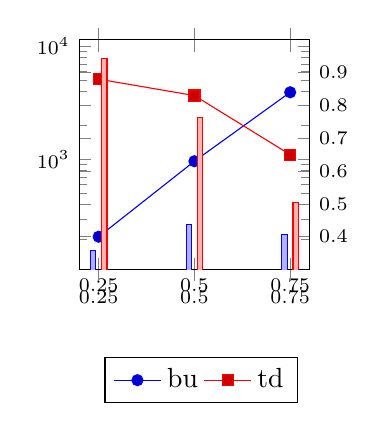
\begin{tikzpicture}
	\begin{axis}
		 [
			width=4.5cm,
			height=4.5cm,
			ymin= 0.3,
			ymax = 1,
			%grid,
			%ymode = log,
			xtick = {0.25,0.5,0.75},
			ytick = {0.4,0.5,0.6,0.7,0.8,0.9},
			%yticklabels = {0.1,0.2,0.3,0.4,0.5,0.6,0.7,0.8,0.9,1.0},
			legend style={at={(0.95,-0.38)}},
			legend columns=4,
			yticklabel pos=right
		 ]
		\addplot+[sharp plot] coordinates
			{(0.25, 0.40) (0.5, 0.63) (0.75, 0.84)};
		\addplot+[sharp plot] coordinates
			{(0.25, 0.88) (0.5, 0.83) (0.75, 0.65)};
		\legend{bu, td}
	\end{axis}
	\begin{axis}
		 [
			width=4.5cm,
			height=4.5cm,
			%grid,
			ymode = log,
			xtick = {0.25,0.5,0.75},
			ytick = {10,100,1000,10000},
			%yticklabels = {0.1,0.2,0.3,0.4,0.5,0.6,0.7,0.8,0.9,1.0},
			legend style={at={(0.95,-0.38)}},
			legend columns=4,
			yticklabel pos=left,
			ybar,
			bar width=2pt,
		 ]
		\addplot+[] coordinates
			{(0.25, 158) (0.5, 268) (0.75, 220)};
		\addplot+[] coordinates
			{(0.25, 7735) (0.5, 2337) (0.75, 415)};
	\end{axis}
\end{tikzpicture}
\caption{}
\label{fig:frac-meta-search-tree}
\end{subfigure}
\caption{(a) average search time per meta search node; 
	(b) average fraction of explored meta search tree} 
\end{figure}



\subsubsection*{Action Set Properties}


\FloatBarrier
\begin{figure*}[ht]

\tiny
\begin{tikzpicture}


\begin{axis}[
width = 7cm,
height=4cm,
enlarge x limits = 0.1,
enlarge y limits = 0.1,
ybar,
bar width=1pt,
ymin = 0,
ymax = 10,
at={(0.0\linewidth,-0.0)},
compat=1.6,
title=c 100,
ylabel=goals 4,
]
\addplot+[ybar, bar shift =-6pt, gray,
]
plot coordinates {
(07, 10)
(08, 10)
(01, 10)
(09, 10)
(06, 10)
(03, 10)
(04, 10)
(05, 10)
(02, 10)
(10, 9)
};
\label{plot:properties_hff_bu}
\addplot+[ybar, bar shift =-3pt, blue,
]
plot coordinates {
(07, 10)
(05, 10)
(04, 10)
(08, 10)
(01, 10)
(09, 10)
(03, 10)
(06, 10)
(02, 10)
(10, 10)
};
\label{plot:properties_hmax_bu}
\addplot+[ybar, bar shift =-4.5pt, purple,
]
plot coordinates {
(07, 10)
(04, 10)
(08, 10)
(09, 9)
(03, 10)
(06, 10)
(05, 10)
(01, 10)
(10, 9)
(02, 10)
};
\label{plot:properties_hmax_td}
\addplot+[ybar, bar shift =-1.5pt, yellow,
]
plot coordinates {
(05, 10)
(08, 10)
(07, 10)
(09, 10)
(03, 10)
(04, 10)
(06, 10)
(01, 10)
(10, 10)
(02, 10)
};
\label{plot:properties_trap_bu}
\addplot+[ybar, bar shift =0pt, orange,
]
plot coordinates {
(04, 10)
(08, 10)
(01, 10)
(09, 10)
(06, 10)
(03, 10)
(07, 10)
(05, 10)
(02, 10)
(10, 10)
};
\label{plot:properties_trap_td}
\addplot+[ybar, bar shift =1.5pt, red,
]
plot coordinates {
(07, 7)
(08, 9)
(09, 6)
(03, 10)
(06, 7)
(04, 9)
(05, 8)
(01, 10)
(10, 5)
(02, 10)
};
\label{plot:properties_hC_td}
\addplot+[ybar, bar shift =3pt, darkgreen,
]
plot coordinates {
(07, 5)
(05, 8)
(04, 10)
(08, 4)
(09, 2)
(03, 10)
(06, 5)
(01, 10)
(02, 10)
(10, 0)
};
\label{plot:properties_hCnr_td}

\end{axis}
\hfill


\begin{axis}[
width = 7cm,
height=4cm,
enlarge x limits = 0.1,
enlarge y limits = 0.1,
ybar,
bar width=1pt,
ymin = 0,
ymax = 10,
at={(0.333333333333\linewidth,-0.0)},
compat=1.6,
title=c 150,
]
\addplot+[ybar, bar shift =-6pt, gray,
]
plot coordinates {
(05, 9)
(04, 10)
(03, 10)
(10, 1)
(02, 10)
(06, 8)
(09, 1)
(08, 2)
(07, 5)
(01, 10)
};
\label{plot:properties_hff_bu}
\addplot+[ybar, bar shift =-3pt, blue,
]
plot coordinates {
(05, 7)
(04, 10)
(03, 10)
(10, 0)
(02, 10)
(08, 1)
(07, 2)
(06, 3)
(01, 10)
(09, 1)
};
\label{plot:properties_hmax_bu}
\addplot+[ybar, bar shift =-4.5pt, purple,
]
plot coordinates {
(05, 9)
(04, 10)
(03, 10)
(10, 0)
(02, 10)
(08, 1)
(07, 3)
(09, 1)
(06, 7)
(01, 10)
};
\label{plot:properties_hmax_td}
\addplot+[ybar, bar shift =-1.5pt, yellow,
]
plot coordinates {
(05, 8)
(04, 9)
(10, 2)
(02, 10)
(09, 2)
(08, 3)
(03, 10)
(07, 5)
(06, 6)
(01, 10)
};
\label{plot:properties_trap_bu}
\addplot+[ybar, bar shift =0pt, orange,
]
plot coordinates {
(05, 10)
(08, 4)
(04, 10)
(03, 10)
(10, 2)
(02, 10)
(06, 8)
(07, 4)
(01, 10)
(09, 3)
};
\label{plot:properties_trap_td}
\addplot+[ybar, bar shift =1.5pt, red,
]
plot coordinates {
(05, 3)
(08, 0)
(04, 5)
(10, 0)
(02, 8)
(03, 5)
(07, 0)
(09, 0)
(06, 1)
(01, 10)
};
\label{plot:properties_hC_td}
\addplot+[ybar, bar shift =3pt, darkgreen,
]
plot coordinates {
(05, 3)
(04, 5)
(10, 0)
(02, 8)
(09, 0)
(08, 0)
(03, 6)
(07, 0)
(06, 0)
(01, 10)
};
\label{plot:properties_hCnr_td}

\end{axis}
\hfill


\begin{axis}[
width = 7cm,
height=4cm,
enlarge x limits = 0.1,
enlarge y limits = 0.1,
ybar,
bar width=1pt,
ymin = 0,
ymax = 10,
at={(0.666666666667\linewidth,-0.0)},
compat=1.6,
title=c 200,
]
\addplot+[ybar, bar shift =-6pt, gray,
]
plot coordinates {
(08, 1)
(02, 10)
(03, 10)
(04, 10)
(07, 2)
(09, 0)
(01, 10)
(06, 6)
(10, 0)
(05, 10)
};
\label{plot:properties_hff_bu}
\addplot+[ybar, bar shift =-3pt, blue,
]
plot coordinates {
(08, 0)
(04, 3)
(01, 10)
(07, 0)
(10, 0)
(03, 8)
(09, 0)
(02, 10)
(06, 0)
(05, 1)
};
\label{plot:properties_hmax_bu}
\addplot+[ybar, bar shift =-4.5pt, purple,
]
plot coordinates {
(08, 6)
(07, 8)
(02, 10)
(06, 9)
(04, 10)
(01, 10)
(03, 10)
(09, 5)
(05, 10)
(10, 2)
};
\label{plot:properties_hmax_td}
\addplot+[ybar, bar shift =-1.5pt, yellow,
]
plot coordinates {
(08, 2)
(07, 3)
(03, 10)
(06, 5)
(04, 10)
(09, 0)
(01, 10)
(02, 10)
(05, 9)
(10, 0)
};
\label{plot:properties_trap_bu}
\addplot+[ybar, bar shift =0pt, orange,
]
plot coordinates {
(08, 7)
(02, 10)
(04, 10)
(07, 7)
(03, 10)
(09, 6)
(01, 10)
(06, 10)
(10, 3)
(05, 10)
};
\label{plot:properties_trap_td}
\addplot+[ybar, bar shift =1.5pt, red,
]
plot coordinates {
(08, 0)
(02, 7)
(03, 3)
(06, 1)
(04, 4)
(01, 10)
(07, 0)
(10, 0)
(09, 0)
(05, 2)
};
\label{plot:properties_hC_td}
\addplot+[ybar, bar shift =3pt, darkgreen,
]
plot coordinates {
(08, 0)
(07, 0)
(06, 1)
(09, 0)
(04, 4)
(10, 0)
(03, 3)
(02, 7)
(01, 10)
(05, 2)
};
\label{plot:properties_hCnr_td}

\end{axis}
\hfill


\begin{axis}[
width = 7cm,
height=4cm,
enlarge x limits = 0.1,
enlarge y limits = 0.1,
ybar,
bar width=1pt,
ymin = 0,
ymax = 10,
at={(0.0\linewidth,-160.0)},
compat=1.6,
ylabel=goals 5,
]
\addplot+[ybar, bar shift =-6pt, gray,
]
plot coordinates {
(01, 10)
(08, 9)
(05, 10)
(03, 10)
(02, 10)
(09, 9)
(04, 10)
(07, 9)
(06, 10)
(10, 9)
};
\label{plot:properties_hff_bu}
\addplot+[ybar, bar shift =-3pt, blue,
]
plot coordinates {
(01, 10)
(08, 9)
(03, 10)
(02, 10)
(09, 9)
(07, 9)
(05, 10)
(04, 10)
(06, 10)
(10, 9)
};
\label{plot:properties_hmax_bu}
\addplot+[ybar, bar shift =-4.5pt, purple,
]
plot coordinates {
(01, 10)
(08, 6)
(03, 10)
(05, 10)
(02, 10)
(09, 6)
(04, 10)
(07, 8)
(06, 10)
(10, 2)
};
\label{plot:properties_hmax_td}
\addplot+[ybar, bar shift =-1.5pt, yellow,
]
plot coordinates {
(01, 10)
(08, 10)
(03, 10)
(02, 10)
(07, 10)
(05, 10)
(04, 10)
(09, 10)
(06, 10)
(10, 10)
};
\label{plot:properties_trap_bu}
\addplot+[ybar, bar shift =0pt, orange,
]
plot coordinates {
(01, 10)
(08, 10)
(03, 10)
(02, 10)
(09, 10)
(04, 10)
(07, 10)
(05, 10)
(06, 10)
(10, 10)
};
\label{plot:properties_trap_td}
\addplot+[ybar, bar shift =1.5pt, red,
]
plot coordinates {
(01, 10)
(08, 6)
(03, 8)
(02, 8)
(09, 5)
(04, 8)
(07, 5)
(06, 4)
(10, 2)
(05, 8)
};
\label{plot:properties_hC_td}
\addplot+[ybar, bar shift =3pt, darkgreen,
]
plot coordinates {
(01, 10)
(08, 1)
(03, 8)
(02, 8)
(09, 1)
(04, 8)
(07, 2)
(05, 6)
(06, 2)
(10, 1)
};
\label{plot:properties_hCnr_td}

\end{axis}
\hfill


\begin{axis}[
width = 7cm,
height=4cm,
enlarge x limits = 0.1,
enlarge y limits = 0.1,
ybar,
bar width=1pt,
ymin = 0,
ymax = 10,
at={(0.333333333333\linewidth,-160.0)},
compat=1.6,
]
\addplot+[ybar, bar shift =-6pt, gray,
]
plot coordinates {
(05, 5)
(06, 2)
(10, 0)
(04, 9)
(01, 10)
(09, 0)
(02, 10)
(08, 1)
(07, 1)
(03, 10)
};
\label{plot:properties_hff_bu}
\addplot+[ybar, bar shift =-3pt, blue,
]
plot coordinates {
(05, 1)
(06, 1)
(10, 0)
(03, 6)
(04, 4)
(01, 10)
(09, 0)
(02, 10)
(07, 1)
(08, 1)
};
\label{plot:properties_hmax_bu}
\addplot+[ybar, bar shift =-4.5pt, purple,
]
plot coordinates {
(05, 7)
(06, 4)
(10, 1)
(03, 10)
(04, 9)
(01, 10)
(09, 1)
(02, 10)
(07, 1)
(08, 1)
};
\label{plot:properties_hmax_td}
\addplot+[ybar, bar shift =-1.5pt, yellow,
]
plot coordinates {
(05, 6)
(06, 2)
(10, 1)
(04, 10)
(01, 10)
(09, 1)
(02, 10)
(08, 1)
(07, 1)
(03, 10)
};
\label{plot:properties_trap_bu}
\addplot+[ybar, bar shift =0pt, orange,
]
plot coordinates {
(05, 8)
(06, 4)
(10, 2)
(03, 10)
(04, 10)
(01, 10)
(09, 2)
(02, 10)
(08, 2)
(07, 2)
};
\label{plot:properties_trap_td}
\addplot+[ybar, bar shift =1.5pt, red,
]
plot coordinates {
(05, 0)
(06, 0)
(10, 0)
(03, 3)
(04, 1)
(01, 10)
(09, 0)
(02, 7)
(08, 0)
(07, 0)
};
\label{plot:properties_hC_td}
\addplot+[ybar, bar shift =3pt, darkgreen,
]
plot coordinates {
(05, 0)
(06, 0)
(10, 0)
(04, 2)
(01, 10)
(09, 0)
(02, 7)
(07, 0)
(08, 0)
(03, 4)
};
\label{plot:properties_hCnr_td}

\end{axis}
\hfill


\begin{axis}[
width = 7cm,
height=4cm,
enlarge x limits = 0.1,
enlarge y limits = 0.1,
ybar,
bar width=1pt,
ymin = 0,
ymax = 10,
at={(0.666666666667\linewidth,-160.0)},
compat=1.6,
]
\addplot+[ybar, bar shift =-6pt, gray,
]
plot coordinates {
(03, 10)
(04, 7)
(05, 3)
(09, 0)
(01, 10)
(02, 10)
(08, 0)
(06, 1)
(10, 0)
(07, 0)
};
\label{plot:properties_hff_bu}
\addplot+[ybar, bar shift =-3pt, blue,
]
plot coordinates {
(03, 1)
(04, 0)
(05, 0)
(09, 0)
(01, 8)
(02, 1)
(08, 0)
(06, 0)
(10, 0)
(07, 0)
};
\label{plot:properties_hmax_bu}
\addplot+[ybar, bar shift =-4.5pt, purple,
]
plot coordinates {
(03, 5)
(04, 3)
(05, 1)
(09, 0)
(01, 9)
(08, 0)
(02, 8)
(06, 2)
(10, 0)
(07, 1)
};
\label{plot:properties_hmax_td}
\addplot+[ybar, bar shift =-1.5pt, yellow,
]
plot coordinates {
(03, 9)
(04, 6)
(05, 1)
(09, 0)
(01, 10)
(02, 10)
(08, 0)
(06, 1)
(10, 0)
(07, 0)
};
\label{plot:properties_trap_bu}
\addplot+[ybar, bar shift =0pt, orange,
]
plot coordinates {
(03, 10)
(04, 9)
(05, 4)
(09, 2)
(01, 10)
(02, 10)
(08, 2)
(06, 4)
(10, 1)
(07, 4)
};
\label{plot:properties_trap_td}
\addplot+[ybar, bar shift =1.5pt, red,
]
plot coordinates {
(03, 2)
(04, 1)
(05, 0)
(09, 0)
(01, 10)
(08, 0)
(02, 6)
(07, 0)
(06, 0)
(10, 0)
};
\label{plot:properties_hC_td}
\addplot+[ybar, bar shift =3pt, darkgreen,
]
plot coordinates {
(03, 2)
(04, 1)
(05, 0)
(09, 0)
(01, 10)
(02, 6)
(08, 0)
(06, 0)
(10, 0)
(07, 0)
};
\label{plot:properties_hCnr_td}

\end{axis}
\hfill


\begin{axis}[
width = 7cm,
height=4cm,
enlarge x limits = 0.1,
enlarge y limits = 0.1,
ybar,
bar width=1pt,
ymin = 0,
ymax = 10,
at={(0.0\linewidth,-320.0)},
compat=1.6,
ylabel=goals 6,
]
\addplot+[ybar, bar shift =-6pt, gray,
]
plot coordinates {
(08, 2)
(09, 2)
(01, 10)
(10, 2)
(06, 5)
(04, 8)
(07, 4)
(05, 5)
(02, 9)
(03, 8)
};
\label{plot:properties_hff_bu}
\addplot+[ybar, bar shift =-3pt, blue,
]
plot coordinates {
(06, 3)
(08, 3)
(09, 2)
(01, 10)
(10, 2)
(04, 8)
(05, 5)
(07, 3)
(02, 9)
(03, 8)
};
\label{plot:properties_hmax_bu}
\addplot+[ybar, bar shift =-4.5pt, purple,
]
plot coordinates {
(08, 2)
(09, 2)
(01, 10)
(10, 2)
(06, 2)
(04, 8)
(02, 9)
(05, 5)
(07, 2)
(03, 8)
};
\label{plot:properties_hmax_td}
\addplot+[ybar, bar shift =-1.5pt, yellow,
]
plot coordinates {
(08, 8)
(09, 8)
(01, 10)
(10, 8)
(06, 9)
(04, 10)
(02, 10)
(05, 9)
(07, 8)
(03, 10)
};
\label{plot:properties_trap_bu}
\addplot+[ybar, bar shift =0pt, orange,
]
plot coordinates {
(08, 8)
(09, 8)
(01, 10)
(10, 7)
(06, 7)
(04, 8)
(07, 8)
(02, 10)
(05, 7)
(03, 8)
};
\label{plot:properties_trap_td}
\addplot+[ybar, bar shift =1.5pt, red,
]
plot coordinates {
(08, 4)
(09, 3)
(01, 10)
(10, 3)
(06, 2)
(04, 4)
(05, 3)
(07, 3)
(03, 3)
(02, 6)
};
\label{plot:properties_hC_td}
\addplot+[ybar, bar shift =3pt, darkgreen,
]
plot coordinates {
(06, 2)
(08, 1)
(09, 1)
(01, 10)
(10, 0)
(04, 3)
(05, 3)
(07, 2)
(02, 8)
(03, 3)
};
\label{plot:properties_hCnr_td}

\end{axis}
\hfill


\begin{axis}[
width = 7cm,
height=4cm,
enlarge x limits = 0.1,
enlarge y limits = 0.1,
ybar,
bar width=1pt,
ymin = 0,
ymax = 10,
at={(0.333333333333\linewidth,-320.0)},
compat=1.6,
]
\addplot+[ybar, bar shift =-6pt, gray,
]
plot coordinates {
(06, 1)
(10, 0)
(03, 9)
(05, 3)
(07, 1)
(08, 1)
(02, 10)
(09, 0)
(01, 10)
(04, 7)
};
\label{plot:properties_hff_bu}
\addplot+[ybar, bar shift =-3pt, blue,
]
plot coordinates {
(06, 0)
(10, 0)
(05, 1)
(07, 0)
(08, 0)
(02, 3)
(09, 0)
(01, 5)
(04, 2)
(03, 2)
};
\label{plot:properties_hmax_bu}
\addplot+[ybar, bar shift =-4.5pt, purple,
]
plot coordinates {
(06, 1)
(10, 0)
(03, 5)
(05, 2)
(08, 0)
(07, 0)
(02, 5)
(09, 0)
(01, 5)
(04, 3)
};
\label{plot:properties_hmax_td}
\addplot+[ybar, bar shift =-1.5pt, yellow,
]
plot coordinates {
(06, 2)
(10, 2)
(05, 2)
(08, 2)
(07, 2)
(02, 10)
(09, 2)
(01, 10)
(03, 7)
(04, 4)
};
\label{plot:properties_trap_bu}
\addplot+[ybar, bar shift =0pt, orange,
]
plot coordinates {
(06, 3)
(10, 1)
(03, 7)
(05, 3)
(08, 2)
(07, 2)
(02, 10)
(09, 2)
(01, 10)
(04, 6)
};
\label{plot:properties_trap_td}
\addplot+[ybar, bar shift =1.5pt, red,
]
plot coordinates {
(06, 0)
(10, 0)
(05, 0)
(08, 0)
(07, 0)
(02, 4)
(09, 0)
(01, 9)
(04, 0)
(03, 1)
};
\label{plot:properties_hC_td}
\addplot+[ybar, bar shift =3pt, darkgreen,
]
plot coordinates {
(06, 0)
(10, 0)
(03, 2)
(05, 0)
(07, 0)
(08, 0)
(02, 4)
(09, 0)
(01, 9)
(04, 0)
};
\label{plot:properties_hCnr_td}

\end{axis}
\hfill


\begin{axis}[
width = 7cm,
height=4cm,
enlarge x limits = 0.1,
enlarge y limits = 0.1,
ybar,
bar width=1pt,
ymin = 0,
ymax = 10,
at={(0.666666666667\linewidth,-320.0)},
compat=1.6,
]
\addplot+[ybar, bar shift =-6pt, gray,
]
plot coordinates {
(02, 8)
(01, 10)
(04, 3)
(03, 4)
(06, 1)
(10, 0)
(05, 3)
(09, 0)
(08, 0)
(07, 0)
};
\label{plot:properties_hff_bu}
\addplot+[ybar, bar shift =-3pt, blue,
]
plot coordinates {
(02, 1)
(01, 2)
(04, 0)
(03, 0)
(07, 0)
(08, 0)
(06, 0)
(10, 0)
(05, 0)
(09, 0)
};
\label{plot:properties_hmax_bu}
\addplot+[ybar, bar shift =-4.5pt, purple,
]
plot coordinates {
(02, 2)
(01, 2)
(04, 0)
(03, 1)
(08, 0)
(06, 0)
(10, 0)
(05, 0)
(09, 0)
(07, 0)
};
\label{plot:properties_hmax_td}
\addplot+[ybar, bar shift =-1.5pt, yellow,
]
plot coordinates {
(02, 10)
(01, 10)
(06, 1)
(04, 4)
(03, 5)
(08, 0)
(10, 0)
(05, 2)
(09, 0)
(07, 0)
};
\label{plot:properties_trap_bu}
\addplot+[ybar, bar shift =0pt, orange,
]
plot coordinates {
(02, 10)
(01, 10)
(04, 7)
(03, 7)
(07, 3)
(06, 4)
(10, 2)
(05, 4)
(09, 2)
(08, 2)
};
\label{plot:properties_trap_td}
\addplot+[ybar, bar shift =1.5pt, red,
]
plot coordinates {
(02, 3)
(10, 0)
(04, 0)
(03, 0)
(08, 0)
(06, 0)
(05, 0)
(09, 0)
(01, 10)
(07, 0)
};
\label{plot:properties_hC_td}
\addplot+[ybar, bar shift =3pt, darkgreen,
]
plot coordinates {
(02, 3)
(04, 0)
(03, 0)
(08, 0)
(06, 0)
(10, 0)
(05, 0)
(09, 0)
(01, 10)
(07, 0)
};
\label{plot:properties_hCnr_td}

\end{axis}
\hfill

\node[draw] (test) at (8,-8) {
\ref{plot:properties_hff_bu} properties-hff-bu
\ref{plot:properties_hmax_bu} properties-hmax-bu
\ref{plot:properties_hmax_td} properties-hmax-td
\ref{plot:properties_trap_bu} properties-trap-bu
\ref{plot:properties_trap_td} properties-trap-td
\ref{plot:properties_hC_td} properties-hC-td
\ref{plot:properties_hCnr_td} properties-hCnr-td
};

\end{tikzpicture}
\hfill

\caption{nomystery}
\end{figure*}


\begin{figure*}[ht]

\tiny
\begin{tikzpicture}


\begin{axis}[
width = 7cm,
height=4cm,
enlarge x limits = 0.1,
enlarge y limits = 0.1,
ybar,
bar width=1pt,
ymin = 0,
ymax = 10,
at={(0.0\linewidth,-0.0)},
compat=1.6,
title=c 100,
ylabel=goals 4,
]
\addplot+[ybar, bar shift =-6pt, gray,
]
plot coordinates {
(04, 10)
(03, 10)
(02, 10)
(09, 10)
(01, 10)
(08, 10)
(07, 10)
(10, 10)
(06, 10)
(05, 10)
};
\label{plot:properties_hff_bu}
\addplot+[ybar, bar shift =-3pt, blue,
]
plot coordinates {
(04, 10)
(03, 10)
(02, 10)
(09, 10)
(01, 10)
(08, 10)
(07, 10)
(10, 10)
(06, 10)
(05, 10)
};
\label{plot:properties_hmax_bu}
\addplot+[ybar, bar shift =-4.5pt, purple,
]
plot coordinates {
(04, 10)
(03, 10)
(02, 10)
(09, 10)
(01, 10)
(08, 10)
(07, 10)
(10, 10)
(06, 10)
(05, 10)
};
\label{plot:properties_hmax_td}
\addplot+[ybar, bar shift =-1.5pt, yellow,
]
plot coordinates {
(04, 10)
(03, 10)
(02, 10)
(09, 10)
(01, 10)
(08, 10)
(07, 10)
(10, 10)
(06, 10)
(05, 10)
};
\label{plot:properties_trap_bu}
\addplot+[ybar, bar shift =0pt, orange,
]
plot coordinates {
(04, 10)
(03, 10)
(02, 10)
(09, 10)
(01, 10)
(08, 10)
(07, 10)
(10, 10)
(06, 10)
(05, 10)
};
\label{plot:properties_trap_td}
\addplot+[ybar, bar shift =1.5pt, red,
]
plot coordinates {
(04, 10)
(03, 10)
(02, 10)
(09, 9)
(01, 10)
(08, 10)
(07, 10)
(10, 9)
(06, 10)
(05, 10)
};
\label{plot:properties_hC_td}
\addplot+[ybar, bar shift =3pt, darkgreen,
]
plot coordinates {
(04, 10)
(03, 10)
(02, 10)
(09, 7)
(01, 10)
(08, 9)
(07, 10)
(10, 4)
(06, 10)
(05, 10)
};
\label{plot:properties_hCnr_td}

\end{axis}
\hfill


\begin{axis}[
width = 7cm,
height=4cm,
enlarge x limits = 0.1,
enlarge y limits = 0.1,
ybar,
bar width=1pt,
ymin = 0,
ymax = 10,
at={(0.333333333333\linewidth,-0.0)},
compat=1.6,
title=c 150,
]
\addplot+[ybar, bar shift =-6pt, gray,
]
plot coordinates {
(07, 10)
(08, 10)
(09, 10)
(01, 10)
(02, 10)
(03, 10)
(04, 10)
(05, 10)
(06, 10)
(10, 10)
};
\label{plot:properties_hff_bu}
\addplot+[ybar, bar shift =-3pt, blue,
]
plot coordinates {
(07, 8)
(08, 6)
(09, 3)
(01, 10)
(04, 10)
(02, 10)
(03, 10)
(05, 10)
(10, 1)
(06, 10)
};
\label{plot:properties_hmax_bu}
\addplot+[ybar, bar shift =-4.5pt, purple,
]
plot coordinates {
(07, 10)
(08, 9)
(09, 8)
(01, 10)
(02, 10)
(03, 10)
(04, 10)
(05, 10)
(06, 10)
(10, 4)
};
\label{plot:properties_hmax_td}
\addplot+[ybar, bar shift =-1.5pt, yellow,
]
plot coordinates {
(07, 10)
(08, 9)
(09, 9)
(01, 10)
(02, 10)
(03, 10)
(04, 10)
(05, 10)
(06, 10)
(10, 9)
};
\label{plot:properties_trap_bu}
\addplot+[ybar, bar shift =0pt, orange,
]
plot coordinates {
(07, 10)
(08, 10)
(09, 10)
(01, 10)
(02, 10)
(03, 10)
(04, 10)
(05, 10)
(06, 10)
(10, 10)
};
\label{plot:properties_trap_td}
\addplot+[ybar, bar shift =1.5pt, red,
]
plot coordinates {
(07, 8)
(08, 6)
(09, 3)
(01, 10)
(04, 10)
(02, 10)
(03, 10)
(05, 10)
(06, 9)
(10, 1)
};
\label{plot:properties_hC_td}
\addplot+[ybar, bar shift =3pt, darkgreen,
]
plot coordinates {
(07, 7)
(08, 6)
(09, 1)
(01, 10)
(02, 10)
(03, 10)
(04, 10)
(05, 10)
(10, 0)
(06, 9)
};
\label{plot:properties_hCnr_td}

\end{axis}
\hfill


\begin{axis}[
width = 7cm,
height=4cm,
enlarge x limits = 0.1,
enlarge y limits = 0.1,
ybar,
bar width=1pt,
ymin = 0,
ymax = 10,
at={(0.666666666667\linewidth,-0.0)},
compat=1.6,
title=c 200,
]
\addplot+[ybar, bar shift =-6pt, gray,
]
plot coordinates {
(07, 10)
(04, 10)
(05, 10)
(06, 10)
(10, 9)
(03, 10)
(08, 10)
(01, 10)
(09, 10)
(02, 10)
};
\label{plot:properties_hff_bu}
\addplot+[ybar, bar shift =-3pt, blue,
]
plot coordinates {
(08, 0)
(03, 10)
(07, 1)
(05, 7)
(02, 10)
(04, 10)
(10, 0)
(01, 10)
(09, 0)
(06, 4)
};
\label{plot:properties_hmax_bu}
\addplot+[ybar, bar shift =-4.5pt, purple,
]
plot coordinates {
(08, 10)
(04, 10)
(05, 10)
(06, 10)
(10, 8)
(07, 10)
(03, 10)
(01, 10)
(09, 8)
(02, 10)
};
\label{plot:properties_hmax_td}
\addplot+[ybar, bar shift =-1.5pt, yellow,
]
plot coordinates {
(08, 10)
(03, 10)
(05, 10)
(04, 10)
(10, 8)
(02, 10)
(07, 10)
(01, 10)
(09, 9)
(06, 10)
};
\label{plot:properties_trap_bu}
\addplot+[ybar, bar shift =0pt, orange,
]
plot coordinates {
(07, 10)
(04, 10)
(05, 10)
(10, 10)
(03, 10)
(08, 10)
(01, 10)
(09, 10)
(06, 10)
(02, 10)
};
\label{plot:properties_trap_td}
\addplot+[ybar, bar shift =1.5pt, red,
]
plot coordinates {
(08, 7)
(03, 10)
(05, 10)
(04, 10)
(10, 5)
(07, 9)
(02, 10)
(01, 10)
(09, 7)
(06, 10)
};
\label{plot:properties_hC_td}
\addplot+[ybar, bar shift =3pt, darkgreen,
]
plot coordinates {
(03, 10)
(07, 10)
(02, 10)
(04, 10)
(05, 10)
(10, 5)
(08, 8)
(01, 10)
(09, 7)
(06, 10)
};
\label{plot:properties_hCnr_td}

\end{axis}
\hfill


\begin{axis}[
width = 7cm,
height=4cm,
enlarge x limits = 0.1,
enlarge y limits = 0.1,
ybar,
bar width=1pt,
ymin = 0,
ymax = 10,
at={(0.0\linewidth,-160.0)},
compat=1.6,
ylabel=goals 5,
]
\addplot+[ybar, bar shift =-6pt, gray,
]
plot coordinates {
(08, 10)
(04, 10)
(09, 10)
(01, 10)
(06, 10)
(07, 10)
(02, 10)
(03, 10)
(05, 10)
(10, 10)
};
\label{plot:properties_hff_bu}
\addplot+[ybar, bar shift =-3pt, blue,
]
plot coordinates {
(04, 10)
(08, 10)
(03, 10)
(09, 10)
(01, 10)
(06, 10)
(07, 10)
(02, 10)
(05, 10)
(10, 9)
};
\label{plot:properties_hmax_bu}
\addplot+[ybar, bar shift =-4.5pt, purple,
]
plot coordinates {
(06, 10)
(09, 7)
(07, 10)
(02, 10)
(04, 10)
(03, 10)
(05, 10)
(08, 10)
(10, 4)
(01, 10)
};
\label{plot:properties_hmax_td}
\addplot+[ybar, bar shift =-1.5pt, yellow,
]
plot coordinates {
(03, 10)
(08, 10)
(01, 10)
(09, 10)
(07, 10)
(04, 10)
(06, 10)
(05, 10)
(10, 10)
(02, 10)
};
\label{plot:properties_trap_bu}
\addplot+[ybar, bar shift =0pt, orange,
]
plot coordinates {
(04, 10)
(03, 10)
(08, 10)
(01, 10)
(06, 10)
(09, 10)
(07, 10)
(05, 10)
(10, 10)
(02, 10)
};
\label{plot:properties_trap_td}
\addplot+[ybar, bar shift =1.5pt, red,
]
plot coordinates {
(08, 9)
(04, 10)
(01, 10)
(06, 10)
(09, 8)
(03, 10)
(07, 9)
(05, 9)
(02, 10)
(10, 8)
};
\label{plot:properties_hC_td}
\addplot+[ybar, bar shift =3pt, darkgreen,
]
plot coordinates {
(08, 7)
(09, 1)
(01, 10)
(07, 7)
(04, 10)
(03, 10)
(06, 9)
(05, 10)
(10, 0)
(02, 10)
};
\label{plot:properties_hCnr_td}

\end{axis}
\hfill


\begin{axis}[
width = 7cm,
height=4cm,
enlarge x limits = 0.1,
enlarge y limits = 0.1,
ybar,
bar width=1pt,
ymin = 0,
ymax = 10,
at={(0.333333333333\linewidth,-160.0)},
compat=1.6,
]
\addplot+[ybar, bar shift =-6pt, gray,
]
plot coordinates {
(02, 10)
(05, 10)
(10, 3)
(04, 10)
(07, 7)
(06, 9)
(09, 3)
(01, 10)
(08, 6)
(03, 10)
};
\label{plot:properties_hff_bu}
\addplot+[ybar, bar shift =-3pt, blue,
]
plot coordinates {
(02, 10)
(10, 0)
(05, 5)
(04, 7)
(07, 1)
(06, 3)
(09, 0)
(01, 10)
(08, 0)
(03, 10)
};
\label{plot:properties_hmax_bu}
\addplot+[ybar, bar shift =-4.5pt, purple,
]
plot coordinates {
(02, 10)
(05, 10)
(10, 2)
(04, 10)
(07, 7)
(06, 9)
(09, 2)
(01, 10)
(08, 4)
(03, 10)
};
\label{plot:properties_hmax_td}
\addplot+[ybar, bar shift =-1.5pt, yellow,
]
plot coordinates {
(02, 10)
(10, 5)
(05, 10)
(04, 10)
(07, 9)
(06, 10)
(09, 8)
(01, 10)
(08, 8)
(03, 10)
};
\label{plot:properties_trap_bu}
\addplot+[ybar, bar shift =0pt, orange,
]
plot coordinates {
(02, 10)
(10, 7)
(05, 10)
(04, 10)
(07, 10)
(06, 10)
(09, 10)
(01, 10)
(08, 10)
(03, 10)
};
\label{plot:properties_trap_td}
\addplot+[ybar, bar shift =1.5pt, red,
]
plot coordinates {
(02, 10)
(10, 1)
(05, 6)
(04, 10)
(07, 2)
(06, 4)
(09, 1)
(01, 10)
(08, 2)
(03, 10)
};
\label{plot:properties_hC_td}
\addplot+[ybar, bar shift =3pt, darkgreen,
]
plot coordinates {
(02, 10)
(10, 1)
(05, 8)
(04, 10)
(07, 2)
(06, 4)
(09, 1)
(01, 10)
(08, 2)
(03, 10)
};
\label{plot:properties_hCnr_td}

\end{axis}
\hfill


\begin{axis}[
width = 7cm,
height=4cm,
enlarge x limits = 0.1,
enlarge y limits = 0.1,
ybar,
bar width=1pt,
ymin = 0,
ymax = 10,
at={(0.666666666667\linewidth,-160.0)},
compat=1.6,
]
\addplot+[ybar, bar shift =-6pt, gray,
]
plot coordinates {
(02, 10)
(05, 10)
(04, 10)
(07, 9)
(06, 10)
(10, 8)
(03, 10)
(09, 9)
(01, 10)
(08, 9)
};
\label{plot:properties_hff_bu}
\addplot+[ybar, bar shift =-3pt, blue,
]
plot coordinates {
(03, 3)
(02, 7)
(05, 0)
(04, 0)
(07, 0)
(06, 0)
(10, 0)
(09, 0)
(01, 10)
(08, 0)
};
\label{plot:properties_hmax_bu}
\addplot+[ybar, bar shift =-4.5pt, purple,
]
plot coordinates {
(03, 10)
(02, 10)
(05, 10)
(04, 10)
(07, 9)
(06, 10)
(10, 8)
(09, 9)
(01, 10)
(08, 9)
};
\label{plot:properties_hmax_td}
\addplot+[ybar, bar shift =-1.5pt, yellow,
]
plot coordinates {
(07, 9)
(03, 10)
(02, 10)
(10, 6)
(05, 10)
(04, 10)
(06, 10)
(09, 7)
(01, 10)
(08, 8)
};
\label{plot:properties_trap_bu}
\addplot+[ybar, bar shift =0pt, orange,
]
plot coordinates {
(03, 10)
(02, 10)
(05, 10)
(04, 10)
(07, 10)
(06, 10)
(10, 9)
(09, 10)
(01, 10)
(08, 10)
};
\label{plot:properties_trap_td}
\addplot+[ybar, bar shift =1.5pt, red,
]
plot coordinates {
(03, 10)
(02, 10)
(10, 5)
(05, 9)
(04, 10)
(07, 6)
(06, 8)
(09, 5)
(01, 10)
(08, 6)
};
\label{plot:properties_hC_td}
\addplot+[ybar, bar shift =3pt, darkgreen,
]
plot coordinates {
(03, 10)
(02, 10)
(10, 5)
(05, 9)
(04, 10)
(07, 6)
(06, 8)
(09, 5)
(01, 10)
(08, 6)
};
\label{plot:properties_hCnr_td}

\end{axis}
\hfill


\begin{axis}[
width = 7cm,
height=4cm,
enlarge x limits = 0.1,
enlarge y limits = 0.1,
ybar,
bar width=1pt,
ymin = 0,
ymax = 10,
at={(0.0\linewidth,-320.0)},
compat=1.6,
ylabel=goals 6,
]
\addplot+[ybar, bar shift =-6pt, gray,
]
plot coordinates {
(10, 7)
(09, 8)
(02, 10)
(05, 10)
(03, 10)
(06, 10)
(01, 10)
(08, 9)
(07, 9)
(04, 10)
};
\label{plot:properties_hff_bu}
\addplot+[ybar, bar shift =-3pt, blue,
]
plot coordinates {
(10, 5)
(05, 10)
(04, 10)
(07, 9)
(06, 9)
(01, 10)
(02, 10)
(09, 7)
(08, 7)
(03, 10)
};
\label{plot:properties_hmax_bu}
\addplot+[ybar, bar shift =-4.5pt, purple,
]
plot coordinates {
(10, 0)
(02, 10)
(05, 9)
(03, 10)
(09, 1)
(01, 10)
(08, 2)
(07, 5)
(06, 9)
(04, 10)
};
\label{plot:properties_hmax_td}
\addplot+[ybar, bar shift =-1.5pt, yellow,
]
plot coordinates {
(10, 10)
(04, 10)
(05, 10)
(07, 10)
(06, 10)
(01, 10)
(02, 10)
(09, 10)
(08, 10)
(03, 10)
};
\label{plot:properties_trap_bu}
\addplot+[ybar, bar shift =0pt, orange,
]
plot coordinates {
(10, 10)
(09, 10)
(02, 10)
(07, 10)
(05, 10)
(03, 10)
(06, 10)
(01, 10)
(08, 10)
(04, 10)
};
\label{plot:properties_trap_td}
\addplot+[ybar, bar shift =1.5pt, red,
]
plot coordinates {
(10, 0)
(05, 8)
(04, 7)
(07, 3)
(06, 4)
(02, 9)
(09, 1)
(01, 10)
(08, 1)
(03, 8)
};
\label{plot:properties_hC_td}
\addplot+[ybar, bar shift =3pt, darkgreen,
]
plot coordinates {
(10, 0)
(09, 0)
(05, 4)
(07, 0)
(06, 2)
(01, 10)
(02, 10)
(08, 0)
(03, 10)
(04, 7)
};
\label{plot:properties_hCnr_td}

\end{axis}
\hfill


\begin{axis}[
width = 7cm,
height=4cm,
enlarge x limits = 0.1,
enlarge y limits = 0.1,
ybar,
bar width=1pt,
ymin = 0,
ymax = 10,
at={(0.333333333333\linewidth,-320.0)},
compat=1.6,
]
\addplot+[ybar, bar shift =-6pt, gray,
]
plot coordinates {
(10, 2)
(02, 10)
(03, 10)
(08, 3)
(01, 10)
(06, 5)
(07, 3)
(09, 2)
(04, 9)
(05, 8)
};
\label{plot:properties_hff_bu}
\addplot+[ybar, bar shift =-3pt, blue,
]
plot coordinates {
(10, 0)
(02, 2)
(03, 0)
(08, 0)
(01, 7)
(09, 0)
(06, 0)
(07, 0)
(04, 0)
(05, 0)
};
\label{plot:properties_hmax_bu}
\addplot+[ybar, bar shift =-4.5pt, purple,
]
plot coordinates {
(10, 3)
(02, 9)
(03, 9)
(08, 3)
(01, 8)
(09, 3)
(06, 5)
(07, 3)
(04, 8)
(05, 7)
};
\label{plot:properties_hmax_td}
\addplot+[ybar, bar shift =-1.5pt, yellow,
]
plot coordinates {
(10, 4)
(02, 10)
(03, 10)
(08, 6)
(01, 10)
(09, 5)
(06, 10)
(07, 7)
(04, 10)
(05, 10)
};
\label{plot:properties_trap_bu}
\addplot+[ybar, bar shift =0pt, orange,
]
plot coordinates {
(10, 5)
(02, 10)
(03, 10)
(08, 8)
(01, 10)
(06, 10)
(07, 9)
(09, 6)
(04, 10)
(05, 10)
};
\label{plot:properties_trap_td}
\addplot+[ybar, bar shift =1.5pt, red,
]
plot coordinates {
(10, 0)
(02, 10)
(03, 9)
(08, 2)
(01, 10)
(09, 1)
(06, 0)
(07, 2)
(04, 6)
(05, 5)
};
\label{plot:properties_hC_td}
\addplot+[ybar, bar shift =3pt, darkgreen,
]
plot coordinates {
(10, 0)
(02, 10)
(03, 9)
(08, 2)
(01, 10)
(09, 1)
(06, 1)
(07, 2)
(04, 7)
(05, 5)
};
\label{plot:properties_hCnr_td}

\end{axis}
\hfill


\begin{axis}[
width = 7cm,
height=4cm,
enlarge x limits = 0.1,
enlarge y limits = 0.1,
ybar,
bar width=1pt,
ymin = 0,
ymax = 10,
at={(0.666666666667\linewidth,-320.0)},
compat=1.6,
]
\addplot+[ybar, bar shift =-6pt, gray,
]
plot coordinates {
(04, 10)
(05, 10)
(02, 10)
(03, 10)
(06, 9)
(08, 8)
(09, 8)
(01, 10)
(07, 8)
(10, 7)
};
\label{plot:properties_hff_bu}
\addplot+[ybar, bar shift =-3pt, blue,
]
plot coordinates {
(04, 0)
(05, 0)
(02, 0)
(03, 0)
(08, 0)
(09, 0)
(01, 0)
(06, 0)
(07, 0)
(10, 0)
};
\label{plot:properties_hmax_bu}
\addplot+[ybar, bar shift =-4.5pt, purple,
]
plot coordinates {
(04, 2)
(05, 3)
(02, 0)
(03, 2)
(06, 3)
(08, 2)
(09, 3)
(01, 1)
(07, 3)
(10, 2)
};
\label{plot:properties_hmax_td}
\addplot+[ybar, bar shift =-1.5pt, yellow,
]
plot coordinates {
(04, 10)
(05, 10)
(02, 10)
(03, 10)
(08, 6)
(09, 4)
(01, 10)
(06, 10)
(07, 7)
(10, 3)
};
\label{plot:properties_trap_bu}
\addplot+[ybar, bar shift =0pt, orange,
]
plot coordinates {
(04, 10)
(05, 10)
(02, 10)
(03, 10)
(06, 10)
(08, 10)
(09, 9)
(01, 10)
(07, 10)
(10, 8)
};
\label{plot:properties_trap_td}
\addplot+[ybar, bar shift =1.5pt, red,
]
plot coordinates {
(04, 5)
(05, 4)
(02, 9)
(03, 8)
(06, 3)
(08, 0)
(09, 0)
(01, 10)
(07, 1)
(10, 0)
};
\label{plot:properties_hC_td}
\addplot+[ybar, bar shift =3pt, darkgreen,
]
plot coordinates {
(04, 5)
(05, 4)
(02, 9)
(03, 8)
(06, 3)
(08, 0)
(09, 0)
(01, 10)
(07, 1)
(10, 0)
};
\label{plot:properties_hCnr_td}

\end{axis}
\hfill

\node[draw] (test) at (8,-8) {
\ref{plot:properties_hff_bu} properties-hff-bu
\ref{plot:properties_hmax_bu} properties-hmax-bu
\ref{plot:properties_hmax_td} properties-hmax-td
\ref{plot:properties_trap_bu} properties-trap-bu
\ref{plot:properties_trap_td} properties-trap-td
\ref{plot:properties_hC_td} properties-hC-td
\ref{plot:properties_hCnr_td} properties-hCnr-td
};

\end{tikzpicture}
\hfill

\caption{TPP}
\end{figure*}


\begin{figure*}[ht]

\tiny
\begin{tikzpicture}


\begin{axis}[
width = 7cm,
height=4cm,
enlarge x limits = 0.1,
enlarge y limits = 0.1,
ybar,
bar width=1pt,
ymin = 0,
ymax = 10,
at={(0.0\linewidth,-0.0)},
compat=1.6,
title=c 100,
ylabel=goals 05,
]
\addplot+[ybar, bar shift =-6pt, gray,
]
plot coordinates {
(05, 10)
(04, 10)
(06, 9)
(02, 10)
(10, 6)
(01, 10)
(08, 9)
(09, 7)
(03, 10)
(07, 8)
};
\label{plot:properties_hff_bu}
\addplot+[ybar, bar shift =-3pt, blue,
]
plot coordinates {
(06, 8)
(05, 9)
(01, 10)
(02, 10)
(10, 3)
(08, 6)
(09, 5)
(07, 7)
(03, 10)
(04, 9)
};
\label{plot:properties_hmax_bu}
\addplot+[ybar, bar shift =-4.5pt, purple,
]
plot coordinates {
(06, 9)
(10, 3)
(05, 10)
(04, 10)
(01, 10)
(02, 10)
(09, 4)
(08, 5)
(07, 7)
(03, 10)
};
\label{plot:properties_hmax_td}
\addplot+[ybar, bar shift =-1.5pt, yellow,
]
plot coordinates {
(06, 10)
(05, 10)
(04, 10)
(01, 10)
(10, 10)
(02, 10)
(08, 10)
(09, 10)
(07, 10)
(03, 10)
};
\label{plot:properties_trap_bu}
\addplot+[ybar, bar shift =0pt, orange,
]
plot coordinates {
(06, 10)
(05, 10)
(01, 10)
(09, 10)
(10, 10)
(02, 10)
(08, 10)
(07, 10)
(03, 10)
(04, 10)
};
\label{plot:properties_trap_td}
\addplot+[ybar, bar shift =1.5pt, red,
]
plot coordinates {
(05, 10)
(04, 10)
(06, 10)
(01, 10)
(07, 10)
(10, 10)
(02, 10)
(08, 10)
(09, 10)
(03, 10)
};
\label{plot:properties_hC_td}
\addplot+[ybar, bar shift =3pt, darkgreen,
]
plot coordinates {
(06, 10)
(10, 8)
(05, 10)
(01, 10)
(03, 10)
(09, 10)
(02, 10)
(08, 10)
(07, 10)
(04, 10)
};
\label{plot:properties_hCnr_td}

\end{axis}
\hfill


\begin{axis}[
width = 7cm,
height=4cm,
enlarge x limits = 0.1,
enlarge y limits = 0.1,
ybar,
bar width=1pt,
ymin = 0,
ymax = 10,
at={(0.333333333333\linewidth,-0.0)},
compat=1.6,
title=c 150,
]
\addplot+[ybar, bar shift =-6pt, gray,
]
plot coordinates {
(08, 5)
(01, 10)
(09, 5)
(06, 8)
(07, 5)
(04, 9)
(05, 10)
(10, 4)
(02, 10)
(03, 9)
};
\label{plot:properties_hff_bu}
\addplot+[ybar, bar shift =-3pt, blue,
]
plot coordinates {
(01, 10)
(08, 3)
(09, 3)
(06, 3)
(07, 3)
(04, 7)
(05, 4)
(10, 2)
(02, 9)
(03, 8)
};
\label{plot:properties_hmax_bu}
\addplot+[ybar, bar shift =-4.5pt, purple,
]
plot coordinates {
(01, 10)
(08, 4)
(09, 3)
(06, 4)
(07, 2)
(04, 8)
(05, 8)
(10, 2)
(02, 10)
(03, 9)
};
\label{plot:properties_hmax_td}
\addplot+[ybar, bar shift =-1.5pt, yellow,
]
plot coordinates {
(08, 10)
(01, 10)
(09, 10)
(06, 10)
(05, 10)
(07, 10)
(04, 10)
(10, 10)
(02, 10)
(03, 10)
};
\label{plot:properties_trap_bu}
\addplot+[ybar, bar shift =0pt, orange,
]
plot coordinates {
(08, 10)
(01, 10)
(09, 10)
(06, 10)
(07, 10)
(04, 10)
(05, 10)
(10, 10)
(02, 10)
(03, 10)
};
\label{plot:properties_trap_td}
\addplot+[ybar, bar shift =1.5pt, red,
]
plot coordinates {
(08, 10)
(01, 10)
(09, 10)
(06, 10)
(07, 10)
(04, 10)
(05, 10)
(10, 10)
(02, 10)
(03, 10)
};
\label{plot:properties_hC_td}
\addplot+[ybar, bar shift =3pt, darkgreen,
]
plot coordinates {
(01, 10)
(08, 9)
(09, 7)
(06, 10)
(07, 10)
(04, 10)
(05, 10)
(10, 6)
(02, 10)
(03, 10)
};
\label{plot:properties_hCnr_td}

\end{axis}
\hfill


\begin{axis}[
width = 7cm,
height=4cm,
enlarge x limits = 0.1,
enlarge y limits = 0.1,
ybar,
bar width=1pt,
ymin = 0,
ymax = 10,
at={(0.666666666667\linewidth,-0.0)},
compat=1.6,
title=c 200,
]
\addplot+[ybar, bar shift =-6pt, gray,
]
plot coordinates {
(08, 8)
(04, 10)
(05, 10)
(10, 6)
(02, 10)
(03, 10)
(09, 9)
(01, 10)
(06, 7)
(07, 6)
};
\label{plot:properties_hff_bu}
\addplot+[ybar, bar shift =-3pt, blue,
]
plot coordinates {
(04, 3)
(05, 3)
(10, 2)
(02, 7)
(03, 5)
(08, 2)
(09, 2)
(01, 8)
(06, 3)
(07, 2)
};
\label{plot:properties_hmax_bu}
\addplot+[ybar, bar shift =-4.5pt, purple,
]
plot coordinates {
(04, 6)
(05, 4)
(10, 2)
(02, 8)
(03, 8)
(08, 2)
(09, 2)
(01, 9)
(06, 4)
(07, 3)
};
\label{plot:properties_hmax_td}
\addplot+[ybar, bar shift =-1.5pt, yellow,
]
plot coordinates {
(04, 10)
(05, 10)
(10, 10)
(02, 10)
(03, 10)
(08, 10)
(09, 10)
(01, 10)
(06, 10)
(07, 10)
};
\label{plot:properties_trap_bu}
\addplot+[ybar, bar shift =0pt, orange,
]
plot coordinates {
(04, 10)
(05, 10)
(10, 10)
(02, 10)
(03, 10)
(08, 10)
(09, 10)
(01, 10)
(06, 10)
(07, 10)
};
\label{plot:properties_trap_td}
\addplot+[ybar, bar shift =1.5pt, red,
]
plot coordinates {
(04, 10)
(05, 10)
(10, 10)
(02, 10)
(03, 10)
(08, 10)
(09, 10)
(01, 10)
(06, 9)
(07, 10)
};
\label{plot:properties_hC_td}
\addplot+[ybar, bar shift =3pt, darkgreen,
]
plot coordinates {
(04, 10)
(05, 10)
(10, 8)
(02, 10)
(03, 10)
(08, 9)
(09, 9)
(01, 10)
(06, 9)
(07, 10)
};
\label{plot:properties_hCnr_td}

\end{axis}
\hfill


\begin{axis}[
width = 7cm,
height=4cm,
enlarge x limits = 0.1,
enlarge y limits = 0.1,
ybar,
bar width=1pt,
ymin = 0,
ymax = 10,
at={(0.0\linewidth,-160.0)},
compat=1.6,
ylabel=goals 06,
]
\addplot+[ybar, bar shift =-6pt, gray,
]
plot coordinates {
(02, 10)
(03, 10)
(04, 10)
(05, 9)
(10, 7)
(06, 8)
(07, 7)
(08, 8)
(01, 10)
(09, 5)
};
\label{plot:properties_hff_bu}
\addplot+[ybar, bar shift =-3pt, blue,
]
plot coordinates {
(02, 10)
(03, 10)
(04, 7)
(05, 7)
(10, 3)
(06, 7)
(07, 5)
(08, 3)
(01, 10)
(09, 3)
};
\label{plot:properties_hmax_bu}
\addplot+[ybar, bar shift =-4.5pt, purple,
]
plot coordinates {
(02, 10)
(03, 10)
(04, 10)
(05, 9)
(10, 3)
(06, 8)
(07, 7)
(08, 4)
(01, 10)
(09, 3)
};
\label{plot:properties_hmax_td}
\addplot+[ybar, bar shift =-1.5pt, yellow,
]
plot coordinates {
(02, 10)
(03, 10)
(10, 10)
(04, 10)
(05, 10)
(06, 10)
(07, 10)
(08, 10)
(01, 10)
(09, 10)
};
\label{plot:properties_trap_bu}
\addplot+[ybar, bar shift =0pt, orange,
]
plot coordinates {
(02, 10)
(03, 10)
(04, 10)
(05, 10)
(10, 10)
(06, 10)
(07, 10)
(08, 10)
(01, 10)
(09, 10)
};
\label{plot:properties_trap_td}
\addplot+[ybar, bar shift =1.5pt, red,
]
plot coordinates {
(02, 10)
(03, 10)
(04, 10)
(05, 10)
(06, 10)
(07, 10)
(08, 10)
(01, 10)
(09, 10)
(10, 10)
};
\label{plot:properties_hC_td}
\addplot+[ybar, bar shift =3pt, darkgreen,
]
plot coordinates {
(02, 10)
(03, 10)
(10, 9)
(04, 10)
(05, 10)
(06, 10)
(07, 10)
(08, 10)
(01, 10)
(09, 10)
};
\label{plot:properties_hCnr_td}

\end{axis}
\hfill


\begin{axis}[
width = 7cm,
height=4cm,
enlarge x limits = 0.1,
enlarge y limits = 0.1,
ybar,
bar width=1pt,
ymin = 0,
ymax = 10,
at={(0.333333333333\linewidth,-160.0)},
compat=1.6,
]
\addplot+[ybar, bar shift =-6pt, gray,
]
plot coordinates {
(07, 8)
(06, 7)
(01, 10)
(09, 5)
(08, 5)
(03, 10)
(10, 4)
(02, 10)
(05, 9)
(04, 10)
};
\label{plot:properties_hff_bu}
\addplot+[ybar, bar shift =-3pt, blue,
]
plot coordinates {
(07, 3)
(10, 3)
(06, 3)
(01, 10)
(09, 3)
(08, 3)
(03, 6)
(02, 9)
(05, 3)
(04, 4)
};
\label{plot:properties_hmax_bu}
\addplot+[ybar, bar shift =-4.5pt, purple,
]
plot coordinates {
(07, 3)
(06, 3)
(01, 10)
(09, 3)
(08, 3)
(03, 9)
(02, 9)
(05, 5)
(10, 3)
(04, 7)
};
\label{plot:properties_hmax_td}
\addplot+[ybar, bar shift =-1.5pt, yellow,
]
plot coordinates {
(07, 10)
(06, 10)
(01, 10)
(09, 10)
(08, 10)
(03, 10)
(10, 10)
(02, 10)
(05, 10)
(04, 10)
};
\label{plot:properties_trap_bu}
\addplot+[ybar, bar shift =0pt, orange,
]
plot coordinates {
(07, 10)
(06, 10)
(01, 10)
(09, 10)
(08, 10)
(03, 10)
(02, 10)
(05, 10)
(10, 10)
(04, 10)
};
\label{plot:properties_trap_td}
\addplot+[ybar, bar shift =1.5pt, red,
]
plot coordinates {
(07, 10)
(10, 10)
(06, 10)
(01, 10)
(09, 10)
(08, 10)
(03, 10)
(02, 10)
(05, 10)
(04, 10)
};
\label{plot:properties_hC_td}
\addplot+[ybar, bar shift =3pt, darkgreen,
]
plot coordinates {
(07, 10)
(06, 10)
(01, 10)
(09, 9)
(08, 10)
(03, 10)
(02, 10)
(05, 10)
(10, 6)
(04, 10)
};
\label{plot:properties_hCnr_td}

\end{axis}
\hfill


\begin{axis}[
width = 7cm,
height=4cm,
enlarge x limits = 0.1,
enlarge y limits = 0.1,
ybar,
bar width=1pt,
ymin = 0,
ymax = 10,
at={(0.666666666667\linewidth,-160.0)},
compat=1.6,
]
\addplot+[ybar, bar shift =-6pt, gray,
]
plot coordinates {
(08, 4)
(09, 5)
(01, 10)
(07, 7)
(03, 10)
(10, 4)
(04, 10)
(02, 10)
(05, 9)
(06, 5)
};
\label{plot:properties_hff_bu}
\addplot+[ybar, bar shift =-3pt, blue,
]
plot coordinates {
(08, 3)
(01, 7)
(09, 3)
(03, 3)
(06, 3)
(10, 3)
(02, 4)
(05, 3)
(04, 3)
(07, 3)
};
\label{plot:properties_hmax_bu}
\addplot+[ybar, bar shift =-4.5pt, purple,
]
plot coordinates {
(09, 3)
(08, 3)
(03, 5)
(01, 9)
(10, 3)
(02, 5)
(05, 3)
(04, 4)
(07, 3)
(06, 3)
};
\label{plot:properties_hmax_td}
\addplot+[ybar, bar shift =-1.5pt, yellow,
]
plot coordinates {
(01, 10)
(09, 10)
(08, 10)
(07, 10)
(10, 10)
(04, 10)
(02, 10)
(05, 10)
(03, 10)
(06, 10)
};
\label{plot:properties_trap_bu}
\addplot+[ybar, bar shift =0pt, orange,
]
plot coordinates {
(09, 10)
(01, 10)
(08, 10)
(07, 10)
(06, 10)
(10, 10)
(02, 10)
(05, 10)
(03, 10)
(04, 10)
};
\label{plot:properties_trap_td}
\addplot+[ybar, bar shift =1.5pt, red,
]
plot coordinates {
(09, 10)
(08, 10)
(01, 10)
(10, 10)
(02, 10)
(05, 10)
(03, 10)
(04, 10)
(07, 10)
(06, 10)
};
\label{plot:properties_hC_td}
\addplot+[ybar, bar shift =3pt, darkgreen,
]
plot coordinates {
(08, 10)
(09, 9)
(01, 10)
(03, 10)
(10, 7)
(02, 10)
(05, 10)
(04, 10)
(07, 10)
(06, 10)
};
\label{plot:properties_hCnr_td}

\end{axis}
\hfill


\begin{axis}[
width = 7cm,
height=4cm,
enlarge x limits = 0.1,
enlarge y limits = 0.1,
ybar,
bar width=1pt,
ymin = 0,
ymax = 10,
at={(0.0\linewidth,-320.0)},
compat=1.6,
ylabel=goals 07,
]
\addplot+[ybar, bar shift =-6pt, gray,
]
plot coordinates {
(05, 7)
(04, 8)
(07, 3)
(06, 4)
(09, 4)
(01, 10)
(08, 4)
(03, 9)
(02, 10)
(10, 2)
};
\label{plot:properties_hff_bu}
\addplot+[ybar, bar shift =-3pt, blue,
]
plot coordinates {
(05, 1)
(04, 2)
(07, 1)
(06, 1)
(09, 1)
(01, 8)
(08, 1)
(03, 4)
(02, 5)
(10, 1)
};
\label{plot:properties_hmax_bu}
\addplot+[ybar, bar shift =-4.5pt, purple,
]
plot coordinates {
(04, 2)
(07, 1)
(06, 1)
(09, 1)
(01, 8)
(08, 1)
(05, 3)
(03, 5)
(02, 6)
(10, 1)
};
\label{plot:properties_hmax_td}
\addplot+[ybar, bar shift =-1.5pt, yellow,
]
plot coordinates {
(05, 10)
(04, 10)
(07, 10)
(06, 10)
(09, 10)
(01, 10)
(08, 10)
(03, 10)
(02, 10)
(10, 10)
};
\label{plot:properties_trap_bu}
\addplot+[ybar, bar shift =0pt, orange,
]
plot coordinates {
(05, 10)
(04, 10)
(07, 10)
(06, 10)
(09, 10)
(01, 10)
(08, 10)
(03, 10)
(02, 10)
(10, 10)
};
\label{plot:properties_trap_td}
\addplot+[ybar, bar shift =1.5pt, red,
]
plot coordinates {
(05, 10)
(04, 10)
(07, 10)
(06, 10)
(09, 10)
(01, 10)
(08, 10)
(03, 10)
(02, 10)
(10, 10)
};
\label{plot:properties_hC_td}
\addplot+[ybar, bar shift =3pt, darkgreen,
]
plot coordinates {
(04, 10)
(07, 10)
(06, 10)
(09, 7)
(01, 10)
(08, 8)
(05, 10)
(03, 10)
(02, 10)
(10, 6)
};
\label{plot:properties_hCnr_td}

\end{axis}
\hfill


\begin{axis}[
width = 7cm,
height=4cm,
enlarge x limits = 0.1,
enlarge y limits = 0.1,
ybar,
bar width=1pt,
ymin = 0,
ymax = 10,
at={(0.333333333333\linewidth,-320.0)},
compat=1.6,
]
\addplot+[ybar, bar shift =-6pt, gray,
]
plot coordinates {
(08, 4)
(09, 3)
(01, 10)
(03, 8)
(02, 10)
(04, 9)
(05, 10)
(06, 6)
(10, 2)
(07, 6)
};
\label{plot:properties_hff_bu}
\addplot+[ybar, bar shift =-3pt, blue,
]
plot coordinates {
(01, 3)
(02, 1)
(04, 1)
(03, 1)
(05, 1)
(06, 1)
(10, 1)
(07, 1)
(08, 1)
(09, 1)
};
\label{plot:properties_hmax_bu}
\addplot+[ybar, bar shift =-4.5pt, purple,
]
plot coordinates {
(01, 3)
(08, 1)
(02, 2)
(03, 1)
(04, 1)
(05, 1)
(06, 1)
(10, 1)
(07, 1)
(09, 1)
};
\label{plot:properties_hmax_td}
\addplot+[ybar, bar shift =-1.5pt, yellow,
]
plot coordinates {
(01, 10)
(08, 10)
(02, 10)
(04, 10)
(03, 10)
(05, 10)
(06, 10)
(10, 10)
(07, 10)
(09, 10)
};
\label{plot:properties_trap_bu}
\addplot+[ybar, bar shift =0pt, orange,
]
plot coordinates {
(01, 10)
(02, 10)
(03, 10)
(04, 10)
(05, 10)
(06, 10)
(10, 10)
(07, 10)
(08, 10)
(09, 10)
};
\label{plot:properties_trap_td}
\addplot+[ybar, bar shift =1.5pt, red,
]
plot coordinates {
(01, 10)
(08, 10)
(02, 10)
(03, 10)
(04, 10)
(05, 10)
(06, 10)
(10, 10)
(07, 9)
(09, 10)
};
\label{plot:properties_hC_td}
\addplot+[ybar, bar shift =3pt, darkgreen,
]
plot coordinates {
(08, 9)
(09, 8)
(01, 10)
(03, 10)
(04, 10)
(05, 10)
(02, 10)
(06, 9)
(10, 7)
(07, 9)
};
\label{plot:properties_hCnr_td}

\end{axis}
\hfill


\begin{axis}[
width = 7cm,
height=4cm,
enlarge x limits = 0.1,
enlarge y limits = 0.1,
ybar,
bar width=1pt,
ymin = 0,
ymax = 10,
at={(0.666666666667\linewidth,-320.0)},
compat=1.6,
]
\addplot+[ybar, bar shift =-6pt, gray,
]
plot coordinates {
(08, 4)
(07, 8)
(01, 10)
(09, 5)
(02, 10)
(03, 10)
(04, 10)
(05, 10)
(06, 8)
(10, 2)
};
\label{plot:properties_hff_bu}
\addplot+[ybar, bar shift =-3pt, blue,
]
plot coordinates {
(08, 1)
(07, 1)
(09, 1)
(03, 1)
(05, 1)
(04, 1)
(06, 1)
(02, 1)
(10, 1)
(01, 1)
};
\label{plot:properties_hmax_bu}
\addplot+[ybar, bar shift =-4.5pt, purple,
]
plot coordinates {
(08, 1)
(09, 1)
(03, 1)
(05, 1)
(04, 1)
(06, 1)
(02, 1)
(10, 1)
(07, 1)
(01, 1)
};
\label{plot:properties_hmax_td}
\addplot+[ybar, bar shift =-1.5pt, yellow,
]
plot coordinates {
(08, 10)
(09, 10)
(02, 10)
(03, 10)
(05, 10)
(04, 10)
(06, 10)
(10, 10)
(07, 10)
(01, 10)
};
\label{plot:properties_trap_bu}
\addplot+[ybar, bar shift =0pt, orange,
]
plot coordinates {
(08, 10)
(07, 10)
(01, 10)
(09, 10)
(02, 10)
(03, 10)
(04, 10)
(05, 10)
(06, 10)
(10, 10)
};
\label{plot:properties_trap_td}
\addplot+[ybar, bar shift =1.5pt, red,
]
plot coordinates {
(08, 10)
(01, 10)
(09, 10)
(03, 10)
(05, 10)
(04, 10)
(06, 10)
(02, 10)
(10, 10)
(07, 10)
};
\label{plot:properties_hC_td}
\addplot+[ybar, bar shift =3pt, darkgreen,
]
plot coordinates {
(08, 10)
(09, 9)
(03, 10)
(05, 10)
(04, 10)
(06, 10)
(02, 10)
(10, 8)
(07, 10)
(01, 10)
};
\label{plot:properties_hCnr_td}

\end{axis}
\hfill


\begin{axis}[
width = 7cm,
height=4cm,
enlarge x limits = 0.1,
enlarge y limits = 0.1,
ybar,
bar width=1pt,
ymin = 0,
ymax = 10,
at={(0.0\linewidth,-480.0)},
compat=1.6,
ylabel=goals 08,
]
\addplot+[ybar, bar shift =-6pt, gray,
]
plot coordinates {
(04, 6)
(05, 6)
(02, 10)
(10, 3)
(03, 9)
(08, 3)
(09, 4)
(06, 6)
(07, 4)
(01, 9)
};
\label{plot:properties_hff_bu}
\addplot+[ybar, bar shift =-3pt, blue,
]
plot coordinates {
(04, 3)
(05, 3)
(02, 4)
(10, 3)
(03, 4)
(08, 3)
(09, 3)
(06, 3)
(07, 3)
(01, 8)
};
\label{plot:properties_hmax_bu}
\addplot+[ybar, bar shift =-4.5pt, purple,
]
plot coordinates {
(01, 8)
(04, 5)
(05, 4)
(02, 6)
(10, 3)
(03, 6)
(08, 3)
(09, 3)
(06, 4)
(07, 4)
};
\label{plot:properties_hmax_td}
\addplot+[ybar, bar shift =-1.5pt, yellow,
]
plot coordinates {
(04, 10)
(05, 10)
(02, 10)
(10, 10)
(03, 10)
(08, 10)
(09, 10)
(01, 10)
(06, 10)
(07, 10)
};
\label{plot:properties_trap_bu}
\addplot+[ybar, bar shift =0pt, orange,
]
plot coordinates {
(04, 10)
(05, 10)
(02, 10)
(10, 10)
(03, 10)
(08, 10)
(09, 10)
(06, 10)
(07, 10)
(01, 10)
};
\label{plot:properties_trap_td}
\addplot+[ybar, bar shift =1.5pt, red,
]
plot coordinates {
(04, 10)
(05, 10)
(02, 10)
(10, 10)
(03, 10)
(08, 10)
(09, 10)
(01, 10)
(06, 10)
(07, 10)
};
\label{plot:properties_hC_td}
\addplot+[ybar, bar shift =3pt, darkgreen,
]
plot coordinates {
(04, 10)
(05, 10)
(02, 10)
(10, 4)
(03, 10)
(08, 10)
(09, 8)
(01, 10)
(06, 10)
(07, 10)
};
\label{plot:properties_hCnr_td}

\end{axis}
\hfill


\begin{axis}[
width = 7cm,
height=4cm,
enlarge x limits = 0.1,
enlarge y limits = 0.1,
ybar,
bar width=1pt,
ymin = 0,
ymax = 10,
at={(0.333333333333\linewidth,-480.0)},
compat=1.6,
]
\addplot+[ybar, bar shift =-6pt, gray,
]
plot coordinates {
(02, 10)
(09, 4)
(01, 10)
(08, 3)
(07, 4)
(06, 6)
(10, 2)
(05, 8)
(04, 8)
(03, 10)
};
\label{plot:properties_hff_bu}
\addplot+[ybar, bar shift =-3pt, blue,
]
plot coordinates {
(02, 3)
(09, 2)
(01, 3)
(08, 2)
(07, 2)
(06, 2)
(10, 2)
(05, 2)
(04, 2)
(03, 2)
};
\label{plot:properties_hmax_bu}
\addplot+[ybar, bar shift =-4.5pt, purple,
]
plot coordinates {
(07, 2)
(02, 3)
(09, 2)
(01, 3)
(08, 2)
(06, 2)
(10, 2)
(05, 2)
(04, 3)
(03, 4)
};
\label{plot:properties_hmax_td}
\addplot+[ybar, bar shift =-1.5pt, yellow,
]
plot coordinates {
(02, 10)
(09, 10)
(01, 10)
(08, 10)
(07, 10)
(06, 10)
(10, 10)
(05, 10)
(04, 10)
(03, 10)
};
\label{plot:properties_trap_bu}
\addplot+[ybar, bar shift =0pt, orange,
]
plot coordinates {
(02, 10)
(09, 10)
(01, 10)
(08, 10)
(07, 10)
(06, 10)
(10, 10)
(05, 10)
(04, 10)
(03, 10)
};
\label{plot:properties_trap_td}
\addplot+[ybar, bar shift =1.5pt, red,
]
plot coordinates {
(02, 10)
(09, 9)
(01, 10)
(08, 10)
(07, 10)
(03, 10)
(06, 10)
(10, 9)
(05, 10)
(04, 10)
};
\label{plot:properties_hC_td}
\addplot+[ybar, bar shift =3pt, darkgreen,
]
plot coordinates {
(07, 10)
(02, 10)
(09, 7)
(01, 10)
(08, 8)
(03, 10)
(06, 10)
(10, 3)
(05, 10)
(04, 10)
};
\label{plot:properties_hCnr_td}

\end{axis}
\hfill


\begin{axis}[
width = 7cm,
height=4cm,
enlarge x limits = 0.1,
enlarge y limits = 0.1,
ybar,
bar width=1pt,
ymin = 0,
ymax = 10,
at={(0.666666666667\linewidth,-480.0)},
compat=1.6,
]
\addplot+[ybar, bar shift =-6pt, gray,
]
plot coordinates {
(09, 4)
(03, 9)
(04, 9)
(07, 8)
(08, 5)
(10, 3)
(06, 7)
(01, 10)
(05, 7)
(02, 10)
};
\label{plot:properties_hff_bu}
\addplot+[ybar, bar shift =-3pt, blue,
]
plot coordinates {
(02, 2)
(03, 2)
(05, 2)
(09, 2)
(08, 2)
(06, 2)
(07, 2)
(01, 2)
(10, 2)
(04, 2)
};
\label{plot:properties_hmax_bu}
\addplot+[ybar, bar shift =-4.5pt, purple,
]
plot coordinates {
(03, 2)
(09, 2)
(02, 2)
(05, 2)
(06, 2)
(04, 2)
(08, 2)
(07, 2)
(10, 2)
(01, 2)
};
\label{plot:properties_hmax_td}
\addplot+[ybar, bar shift =-1.5pt, yellow,
]
plot coordinates {
(02, 10)
(01, 10)
(03, 10)
(04, 10)
(08, 10)
(07, 10)
(10, 10)
(06, 10)
(09, 10)
(05, 10)
};
\label{plot:properties_trap_bu}
\addplot+[ybar, bar shift =0pt, orange,
]
plot coordinates {
(03, 10)
(02, 10)
(06, 10)
(01, 10)
(07, 10)
(08, 10)
(10, 10)
(09, 10)
(05, 10)
(04, 10)
};
\label{plot:properties_trap_td}
\addplot+[ybar, bar shift =1.5pt, red,
]
plot coordinates {
(03, 10)
(02, 10)
(06, 10)
(05, 10)
(01, 10)
(07, 10)
(08, 10)
(10, 9)
(09, 9)
(04, 10)
};
\label{plot:properties_hC_td}
\addplot+[ybar, bar shift =3pt, darkgreen,
]
plot coordinates {
(05, 10)
(09, 7)
(06, 10)
(03, 10)
(07, 10)
(08, 9)
(10, 6)
(01, 10)
(04, 10)
(02, 10)
};
\label{plot:properties_hCnr_td}

\end{axis}
\hfill


\begin{axis}[
width = 7cm,
height=4cm,
enlarge x limits = 0.1,
enlarge y limits = 0.1,
ybar,
bar width=1pt,
ymin = 0,
ymax = 10,
at={(0.0\linewidth,-640.0)},
compat=1.6,
ylabel=goals 09,
]
\addplot+[ybar, bar shift =-6pt, gray,
]
plot coordinates {
(02, 10)
(01, 10)
(09, 4)
(08, 4)
(07, 4)
(06, 6)
(10, 4)
(05, 6)
(04, 7)
(03, 8)
};
\label{plot:properties_hff_bu}
\addplot+[ybar, bar shift =-3pt, blue,
]
plot coordinates {
(02, 5)
(01, 6)
(09, 4)
(08, 4)
(07, 4)
(06, 4)
(10, 2)
(05, 4)
(04, 5)
(03, 5)
};
\label{plot:properties_hmax_bu}
\addplot+[ybar, bar shift =-4.5pt, purple,
]
plot coordinates {
(02, 6)
(01, 6)
(09, 4)
(08, 4)
(07, 4)
(06, 4)
(10, 4)
(05, 4)
(04, 5)
(03, 5)
};
\label{plot:properties_hmax_td}
\addplot+[ybar, bar shift =-1.5pt, yellow,
]
plot coordinates {
(02, 10)
(01, 10)
(09, 10)
(05, 10)
(08, 10)
(07, 10)
(06, 10)
(10, 10)
(04, 10)
(03, 10)
};
\label{plot:properties_trap_bu}
\addplot+[ybar, bar shift =0pt, orange,
]
plot coordinates {
(02, 10)
(01, 10)
(09, 10)
(05, 10)
(08, 10)
(07, 10)
(06, 10)
(10, 10)
(04, 10)
(03, 10)
};
\label{plot:properties_trap_td}
\addplot+[ybar, bar shift =1.5pt, red,
]
plot coordinates {
(02, 10)
(01, 10)
(09, 10)
(05, 10)
(08, 9)
(07, 10)
(06, 10)
(10, 10)
(04, 10)
(03, 10)
};
\label{plot:properties_hC_td}
\addplot+[ybar, bar shift =3pt, darkgreen,
]
plot coordinates {
(02, 10)
(01, 10)
(09, 9)
(05, 10)
(08, 9)
(07, 10)
(06, 9)
(10, 9)
(04, 10)
(03, 10)
};
\label{plot:properties_hCnr_td}

\end{axis}
\hfill


\begin{axis}[
width = 7cm,
height=4cm,
enlarge x limits = 0.1,
enlarge y limits = 0.1,
ybar,
bar width=1pt,
ymin = 0,
ymax = 10,
at={(0.333333333333\linewidth,-640.0)},
compat=1.6,
]
\addplot+[ybar, bar shift =-6pt, gray,
]
plot coordinates {
(02, 9)
(05, 7)
(10, 4)
(07, 6)
(03, 8)
(04, 8)
(08, 7)
(01, 10)
(09, 4)
(06, 5)
};
\label{plot:properties_hff_bu}
\addplot+[ybar, bar shift =-3pt, blue,
]
plot coordinates {
(07, 4)
(04, 4)
(03, 4)
(05, 4)
(02, 4)
(10, 2)
(08, 4)
(01, 4)
(09, 4)
(06, 4)
};
\label{plot:properties_hmax_bu}
\addplot+[ybar, bar shift =-4.5pt, purple,
]
plot coordinates {
(01, 4)
(07, 4)
(02, 4)
(04, 4)
(05, 4)
(03, 4)
(10, 4)
(08, 4)
(09, 4)
(06, 4)
};
\label{plot:properties_hmax_td}
\addplot+[ybar, bar shift =-1.5pt, yellow,
]
plot coordinates {
(01, 10)
(07, 10)
(05, 10)
(02, 10)
(10, 10)
(03, 10)
(04, 10)
(08, 10)
(09, 10)
(06, 10)
};
\label{plot:properties_trap_bu}
\addplot+[ybar, bar shift =0pt, orange,
]
plot coordinates {
(02, 10)
(03, 10)
(05, 10)
(10, 10)
(07, 10)
(04, 10)
(08, 10)
(01, 10)
(09, 10)
(06, 10)
};
\label{plot:properties_trap_td}
\addplot+[ybar, bar shift =1.5pt, red,
]
plot coordinates {
(01, 10)
(04, 10)
(07, 10)
(05, 10)
(02, 10)
(10, 10)
(03, 10)
(08, 10)
(09, 10)
(06, 9)
};
\label{plot:properties_hC_td}
\addplot+[ybar, bar shift =3pt, darkgreen,
]
plot coordinates {
(01, 10)
(07, 10)
(02, 10)
(04, 10)
(05, 10)
(03, 10)
(10, 8)
(08, 10)
(09, 9)
(06, 9)
};
\label{plot:properties_hCnr_td}

\end{axis}
\hfill


\begin{axis}[
width = 7cm,
height=4cm,
enlarge x limits = 0.1,
enlarge y limits = 0.1,
ybar,
bar width=1pt,
ymin = 0,
ymax = 10,
at={(0.666666666667\linewidth,-640.0)},
compat=1.6,
]
\addplot+[ybar, bar shift =-6pt, gray,
]
plot coordinates {
(03, 9)
(08, 5)
(09, 4)
(04, 9)
(02, 10)
(07, 4)
(05, 8)
(10, 4)
(06, 4)
(01, 10)
};
\label{plot:properties_hff_bu}
\addplot+[ybar, bar shift =-3pt, blue,
]
plot coordinates {
(08, 4)
(01, 4)
(09, 4)
(06, 4)
(03, 4)
(02, 4)
(07, 4)
(04, 4)
(05, 4)
(10, 2)
};
\label{plot:properties_hmax_bu}
\addplot+[ybar, bar shift =-4.5pt, purple,
]
plot coordinates {
(08, 4)
(09, 4)
(03, 4)
(06, 4)
(02, 4)
(07, 4)
(04, 4)
(05, 4)
(10, 4)
(01, 4)
};
\label{plot:properties_hmax_td}
\addplot+[ybar, bar shift =-1.5pt, yellow,
]
plot coordinates {
(08, 10)
(09, 10)
(03, 10)
(06, 10)
(07, 10)
(02, 10)
(04, 10)
(05, 10)
(10, 10)
(01, 10)
};
\label{plot:properties_trap_bu}
\addplot+[ybar, bar shift =0pt, orange,
]
plot coordinates {
(08, 10)
(01, 10)
(09, 10)
(06, 10)
(03, 10)
(07, 10)
(02, 10)
(04, 10)
(05, 10)
(10, 10)
};
\label{plot:properties_trap_td}
\addplot+[ybar, bar shift =1.5pt, red,
]
plot coordinates {
(03, 10)
(08, 10)
(09, 9)
(06, 9)
(07, 10)
(04, 10)
(05, 10)
(10, 10)
(02, 10)
(01, 10)
};
\label{plot:properties_hC_td}
\addplot+[ybar, bar shift =3pt, darkgreen,
]
plot coordinates {
(08, 10)
(01, 10)
(09, 9)
(03, 10)
(07, 9)
(02, 10)
(04, 10)
(05, 10)
(10, 8)
(06, 9)
};
\label{plot:properties_hCnr_td}

\end{axis}
\hfill

\node[draw] (test) at (8,-14) {
\ref{plot:properties_hff_bu} properties-hff-bu
\ref{plot:properties_hmax_bu} properties-hmax-bu
\ref{plot:properties_hmax_td} properties-hmax-td
\ref{plot:properties_trap_bu} properties-trap-bu
\ref{plot:properties_trap_td} properties-trap-td
\ref{plot:properties_hC_td} properties-hC-td
\ref{plot:properties_hCnr_td} properties-hCnr-td
};

\end{tikzpicture}
\hfill

\caption{rovers}
\end{figure*}
